\chapter{Deep neural regularizers}%
\label{chap:deep neural regularizers}%
\graphicspath{{chapters/deep-neural-regularizers/figures}}%
In \marginnote{\footnotesize \textbf{Contents:}\\\localtableofcontents}the previous chapter, we outlined the historical development of regularizers in imaging.
Starting from classical regularizers based on first principles, such as bounded norm or gradient sparsity of the signal, we highlighted the challenges of manually modeling image statistics and tuning parameters.
This led to the idea of \emph{learning} statistics from data.

In this chapter, we follow this idea by learning a generic deep neural regularizer that prefers structures present in the training data instead of prescribing any particular form of regularizer.
We design a \gls{nn} that maps from the input space, images of size \( \Height \times \Width \), to the real numbers and associate the output with a Gibbs distribution.
This Gibbs distribution is matched to the reference distribution by minimizing the Kullback-Leibler divergence (\cref{def:kullback leibler divergence}).
This chapter largely focuses on developing this idea in the context of \gls{mri} reconstruction, as some of our contributions are specific to this domain.
In particular, we propose a joint nonlinear inversion algorithm for parallel \gls{mri} that utilizes the data-driven regularizer.
However, we also present some results on \gls{ct} to demonstrate the approach's generality.

This chapter is structured as follows:
In~\cref{sec:intro deep neural regularizers} we give an overview of the problems encountered in \gls{mri} imaging and review data-driven reconstruction approaches.
In particular, we discuss approaches to parallel \gls{mri}.
\Cref{sec:discriminative pitfalls} highlights issues with discriminative approaches through a striking example and~\cref{sec:methods} outlines how we solve these problems through a generative approach.
This section encompasses discussion about the motivation behind the architecture of the deep neural regularizer, the probabilistic setup for parameter identification, and the fast joint nonlinear inversion algorithm.
The implementation details and practical considerations discussed in~\cref{ssec:details} are vital for reproducing the results and serve as a reference if anything remains unclear.
We show results on single-coil and multi-coil imaging in~\cref{sec:results deep neural regularizer}.
Additionally, this section focuses on interpretability of the results by visualizing the preferred structures of the regularizer in a data-independent analysis and through uncertainty quantification using the marginal posterior variance.
Further, we demonstrate that the regularizer remains stable when confronted with out-of-distribution data and that our joint nonlinear inversion algorithm yields superior coil sensitivities compared to offline estimation algorithms when few data are available.
Finally, in~\cref{sec:discussion} we discuss the implications and limitations of our approach and conclude that chapter in~\cref{sec:conclusion deep neural regularizer}.

This chapter is based on the following publications:\\
\rule{\linewidth}{.1em}
\fullcite{zach_computed_2021}\\[.2cm]
\fullcite{zach_stable_2023}\\
\rule{\linewidth}{.1em}
Code for training, validation, and visualization, along with pre-trained models, is available at \href{https://github.com/VLOGroup/stable-deep-mri}{https://github.com/VLOGroup/stable-deep-mri}.
A related publication, showing preliminary results of joint nonlinear inversion with diffusion priors, is~\cite{erlacher23}.
\section{Introduction}
\label{sec:intro deep neural regularizers}
\Gls{mri} is a crucial imaging techniques in clinical practice~\cite{Westbrook2018-pj}.
In \gls{mri}, a scanner's receiver coil measures the changes in magnetism of nuclei excited by radiofrequency pulses, and these measurements correspond to Fourier coefficients of the underlying signal via the two-dimensional discrete Fourier transform.
However, populating the observation with frequency data is time consuming and long examination times severely limit patient throughput.
Therefore, extensive research is dedicated to reducing examination time while retaining diagnostic value.

On the hardware side, parallel \gls{mri}~\cite{Roemer1990} exploits spatially varying sensitivities of coil arrays.
This has become standard in clinical systems, but noise amplification limits the potential speed up with classical reconstruction techniques~\cite{Robson2008}.
On the algorithmic side, compressed sensing~\cite{donoho_compressed_2006} and variational approaches enable greater acceleration.
As a prominent example, \gls{tv} regularization has been successfully applied to parallel \gls{mri}~\cite{Knoll2011}.

As shown in the previous chapter, variational approaches with classical penalties like \gls{tv} significantly improve reconstruction.
However, modern data-driven methods such as~\cite{akcakaya_raki_2019,chung_scoremri_2022,hammernik_learning_2017,Narnhofer2019,putzky_irim_2019,zbontar_fastmri_2018,zhou2020dudornet} now outperform these traditional methods.
Data-driven approaches have been applied successfully both as pre-processing steps in Fourier space~\cite{akcakaya_raki_2019} and as post-processing steps in image-space~\cite{zbontar_fastmri_2018}.
\Glspl{vn}~\cite{chen_tnrd_2017,cheng_pdnetworks_2019,hammernik_learning_2017,Kobler2017} unroll an optimization algorithm to imitate the iterative reconstruction schemes, while purely data-driven methods like AUTOMAP~\cite{zhu_image_2018} bypass physical measurement model entirely.

Despite their superior performance, data-driven approaches come with drawbacks that are especially relevant in the context of medical imaging.
First, these discriminative approaches act as a point estimators, mapping data directly to reconstructions.
In contrast, variational approaches enjoy a probabilistic interpretation through Bayes theorem, as discussed in~\cref{sec:variation methods and bayes theorem}.
Data are mapped to a \emph{distribution of reconstructions} which enables uncertainty quantification.
Second, point estimators are typically tied to a particular data likelihood, which is subject to change in \gls{mri} due to different frequency selections or anatomical features.
It has even been shown that reconstruction quality of some data-driven approaches deteriorates with increased data availability~\cite{Antun2020}.
We discuss similar findings in~\cref{sec:discriminative pitfalls}.
Third, these approaches typically rely on vast amounts of paired training data.
In the context of parallel \gls{mri}, this amounts to requiring fully-sampled frequency data which is extremely scarce.
\footnote{%
	The target can be computed from the fully-sampled data, and the input to the reconstruction algorithm can be created retrospectively.
}
In combination, these drawbacks severely hamper the adoption of these methods in clinical practice.

This chapter combines the strengths of modern data-driven methods with the benefits of classical variational approaches by learning a deep neural regularizer that serves as a plug-and-play replacement for classical variational penalties.
The accompanying probabilistic interpretation allows experts to explore the posterior distribution of any reconstruction problem.
We synthesizing realistic images \emph{without} any data, demonstrating that the regularizer encodes the negative log-prior faithfully.
Combining the data-driven regularizer with suitable data-likelihoods for different frequency selections achieves state-of-the-art performance.
Unlike most data-driven approaches, training our model only requires access to a database of reference reconstructions.\footnote{%
	Reference reconstructions are much more abundantly available than the corresponding fully sampled data, and constructing the data from the reconstructions is non-trivial.
}
In addition, we propose a joint nonlinear inversion algorithm based on \gls{ipalm}~\cite{pock_inertial_2016} for parallel \gls{mri}.
A sketch of our proposed approach is shown in~\cref{fig:reco}.
\begin{figure*}
	\centering
	\begin{tikzpicture}[>=latex]
		\def\kspacewidth{2cm}
		\def\kspacexoff{-1.8cm}
		\def\kspaceyoff{0.5cm}
		\def\kspacedx{0.25cm}
		\def\kspacedy{0.25cm}
		\def\sensewidth{0.7cm}
		\def\sensedx{0.1cm}
		\def\sensedy{0.1cm}
		\def\ppad{0.7cm}
		\def\prefix{examples-coils/01}
		\node [inner sep=0, outer sep=0] (kspace1) at (0 * \kspacedx + \kspacexoff, -1 * \kspacedy + \kspaceyoff) {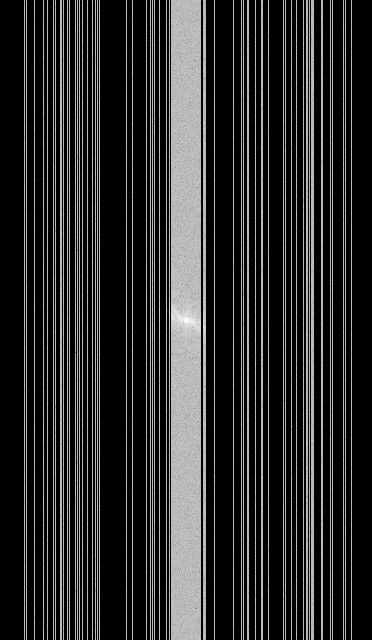
\includegraphics[width=\kspacewidth]{\prefix/kspace_masked/coil_00}};
		\node [inner sep=0, outer sep=0] (kspace2) at (1 * \kspacedx + \kspacexoff, -2 * \kspacedy + \kspaceyoff) {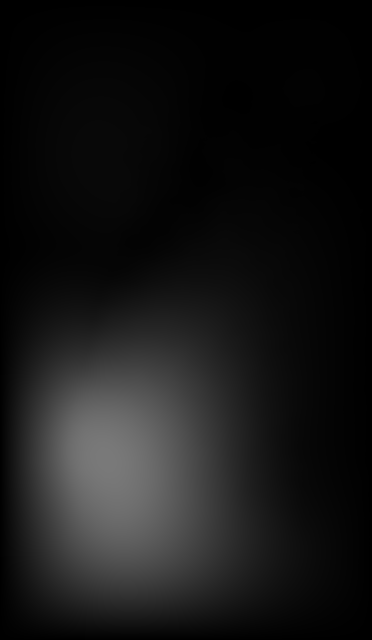
\includegraphics[width=\kspacewidth]{\prefix/kspace_masked/coil_01}};
		\node [inner sep=0, outer sep=0] (kspace3) at (2 * \kspacedx + \kspacexoff, -3 * \kspacedy + \kspaceyoff) {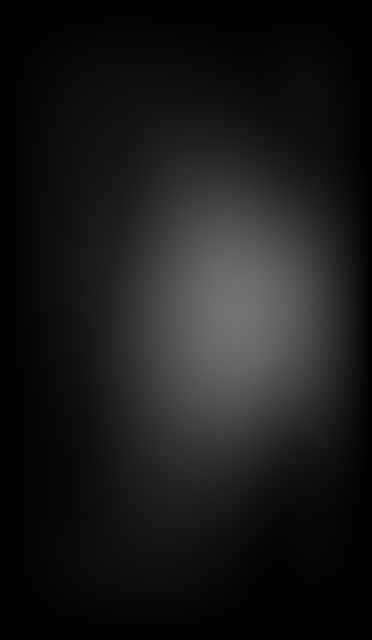
\includegraphics[width=\kspacewidth]{\prefix/kspace_masked/coil_02}};
		\node [inner sep=0, outer sep=0] (kspace6) at (5 * \kspacedx + \kspacexoff, -6 * \kspacedy + \kspaceyoff) {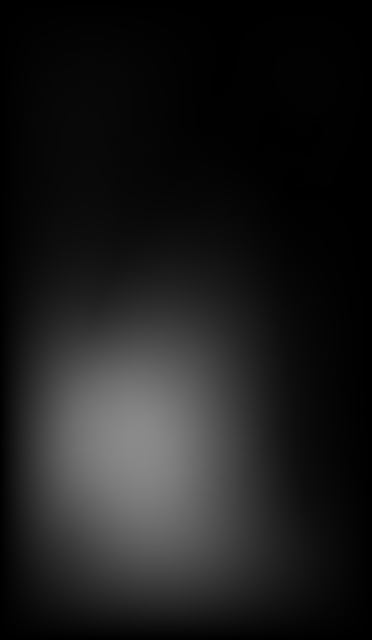
\includegraphics[width=\kspacewidth]{\prefix/kspace_masked/coil_14}};

		\node [below left=-2mm of kspace1.south west] {\( \Adjoint{\Mask}\Data_{\num{1}} \)};
		\node [below left=-2mm of kspace6.south west] {\( \Adjoint{\Mask}\Data_c \)};
		\foreach \i in {1, 2, 3}
		{
			\pgfmathsetmacro{\fr}{\i/4}
			\node at ($(kspace3.south west)!\fr!(kspace6.south west)$) {\( \cdot \)};
			\node at ($(kspace3.north east)!\fr!(kspace6.north east)$) {\( \cdot \)};
		}
		\foreach [count=\i] \which in {00, 20, 40, 90}
		{
			\node[inner sep=0, outer sep=0] (reconstruction\i) at (1cm + \i * \kspacewidth + \i * \ppad, 0.3) {%
				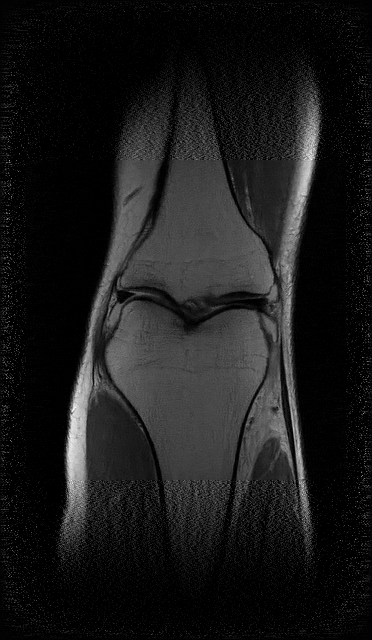
\includegraphics[angle=180,origin=c,width=\kspacewidth]{\prefix/0\which/reconstruction_unnormalized}%
			};
			\node at ($(reconstruction\i.north) + (0, 0.3cm)$) {%
				\ifthenelse{\i=1}{\( x^{0} \)}{%
					\ifthenelse{\i<4}{\( x^{\which} \)}{\( x^{K} \)}
				}%
			};
			\node at (1cm + \i * \kspacewidth + \i * \ppad, -2.5) {%
				\ifthenelse{\i=1}{\( \Sigma^{0} \)}{%
					\ifthenelse{\i<4}{\( \Sigma^{\which} \)}{\( \Sigma^{K} \)}
				}
			};
			\node at (0.9cm + \i * \kspacewidth + \i * \ppad, -1.95) {\( \ddots \)};
			\foreach [count=\isigma] \sigmawhich in {00, 01, 02, 14}
			{
				\ifthenelse{\isigma<4}{\def\offi{\isigma}}{\def\offi{6}}
				\node [inner sep=0, outer sep=0] (sensitivity maps\i\isigma) at (0.7cm + \i * \kspacewidth + \i * \ppad + \offi * \sensedx, -\offi * \sensedy - 1.0cm) {\includegraphics[width=\sensewidth]{\prefix/0\which/coil_\sigmawhich}};
			}
		}
		\node[rounded corners, rectangle, draw, minimum width=0.6cm, minimum height=0.6cm] (initial guess box) at ($(reconstruction1.west) + (-1.2, 0)$) {Naive};
		\draw [<-] (initial guess box) -- ++(-1, 0);
		\draw [->] (initial guess box) -- (reconstruction1);
		\draw [->] (initial guess box) |- (sensitivity maps14.west);
		\foreach \i in {1, 2, 3}
		{
			\pgfmathtruncatemacro{\j}{\i + 1}
			\node [inner sep=0,outer sep=0] (mid\i) at ($(reconstruction\i)!.5!(reconstruction\j)$) {\( \square \)};
			\draw (reconstruction\i) -- (mid\i) [-latex] -- (reconstruction\j);
			\draw [<-,dashed] (mid\i) -- ++(0, 1) node [above] {\( \Data \)};
		}

		\draw [rounded corners, ultra thick, draw=maincolor,] ($(reconstruction1.north west)+(-0.3, 0.6)$) rectangle ($(reconstruction4.south east) + (+0.3, -1.5)$);
		\begin{scope}[shift={(5, 7.5)}]
			\node (nablax) [draw, rounded corners] at (0, 0) {\( \bigl( \argm - L^{-1}_x \Grad H(\,\cdot\,, \Sigma^{k}) \bigr) \)};
			\draw [<-] (nablax) -- (nablax -| -3.8, 0) node [left] {\( x^{k} \)};
			\node (proxU) [draw, rounded corners] at (0, -1.1) {\( \max(0, \argm) \)};
			\draw [->] (proxU) -- (proxU -| 3.8, 0) node [right] {\( x^{k + 1} \)};

			\node (nablaS) [draw, rounded corners] at (0, -2.3) {\( \bigl( \argm - L^{-1}_\Sigma \Grad H(x^{k+1}, \argm)\bigr) \)};
			\draw [<-] (nablaS) -- (nablaS -| -3.8, 0) node [left] {\( \Sigma^{k} \)};
			\node (proxS) [draw, rounded corners] at (0, -3.5) {\( \Adjoint{\DiscreteSineTransform} \bigl( \DiscreteSineTransform(\mu\,\cdot\,) \oslash (\xi + \mu) \bigr) \)};
			\draw [->] (proxS) -- (proxS -| 3.8, 0) node [right] {\( \Sigma^{k + 1} \)};

			\draw [rounded corners, ultra thick, draw=black] ($(nablax.north west -| proxS.south west)+(-0.3, 0.3)$) rectangle ($(proxS.east |- proxS.south)+(0.3, -0.3)$);
			\draw [rounded corners, thick, draw=gray] ($(nablax.north west -| proxS.south west)+(-0.15, 0.15)$) rectangle ($(proxS.east |- proxU.south)+(0.15, -0.15)$);
			\draw [rounded corners, thick, draw=gray] ($(nablaS.north west -| proxS.west)+(-0.15, 0.15)$) rectangle ($(proxS.east |- proxS.south)+(0.15, -0.15)$);
			\draw [<-, dashed] (nablax.east) -- (3.2, 0) node [right] {\( \Data \)};
			\draw [<-, dashed] (nablaS.east) -- (3.2, 0 |- nablaS.east) node [right] {\( \Data \)};
			\draw [->] (nablax) -- (proxU);
			\draw [->] (nablaS) -- (proxS);
		\end{scope}
		\draw [dashed, opacity=0.5] (mid1.north west) to [in=-80,out=110] ($(proxS.south west)+(-0.3, -0.3)$);
		\draw [dashed, opacity=0.5] (mid1.north east) to [in=-110,out=80] ($(proxS.south east)+(0.3, -0.3)$);
	\end{tikzpicture}%
	\caption[Sketch of the joint nonlinear inversion algorithm for parallel MRI]{%
		Sketch of the reconstruction algorithm:
		To jointly reconstruct the spin density \( x \) and the coil sensitivities \( \Sigma = (\sigma_{\num{1}},\sigma_{\num{2}},\dotsc,\sigma_c) \), we impose data-fidelity, image-regularity, and coil-regularity in the iterations of \glsxtrshort{ipalm}~\cite{pock_inertial_2016}.
		The function \( H \) incorporates our data-driven regularizer acting on \( x \).
	}
	\label{fig:reco}
\end{figure*}

\subsection{Parallel MRI}
\label{ssec:parallel imaging intro}
Traditional \gls{mri} encodes the signal location by adjusting precession frequencies using gradient fields in spatial directions.
By exciting the nuclei with a radiofrequency pulse, the entry in the frequency plane encoded by the strength of the gradient fields could be filled.
The introduction of fast gradient-echo and spin-echo sequences, such as echo-planar imaging~\cite{Mansfield1977} or turbo spin-echo~\cite{Hennig1986}, allowed greater portions of the frequency plane to be filled with one excitation pulse.
To achieve even faster imaging, modern \gls{mri} systems employ coil arrays with spatially varying coil sensitivities, as pioneered by Roemer et al.~\cite{Roemer1990} in \num{1990}.
The spatially varying coil sensitivities can be exploited to reduce the number of required spatial modulations.

The following overview of reconstruction algorithms for parallel \gls{mri} draws from the review paper of Blaimer et al.~\cite{Blaimer2004}.
The conceptually simplest reconstruction algorithm for such data is \gls{pils} due to Griswold et al.~\cite{griswold_partially_2000}.
It assumes localized, non-overlapping coil sensitivities and that the entries in the frequency plane are such that the aliased coil images from undersampled reconstructions are non-overlapping.
The idealized situation for a Cartesian frequency selection with acceleration \num{2} is illustrated in~\cref{fig:pils}.
The idealized coil sensitivities of the two receiver coils each cover half of the image and the underlying signals can be recovered exactly.
\begin{figure*}
	\centering
	\begin{tikzpicture}[font=\footnotesize]
		\node at (0, 0) {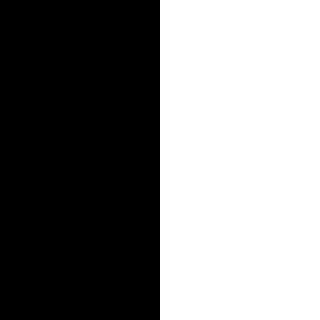
\includegraphics[frame, width=3cm]{../scripts/parallel-mri/s1}};
		\node at (0, -3.2) {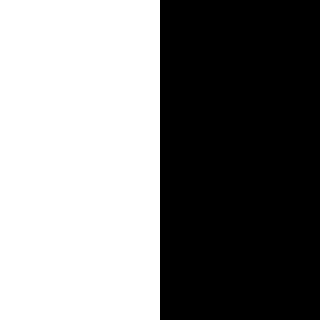
\includegraphics[frame, width=3cm]{../scripts/parallel-mri/s2}};
		\node at (0, -5) {Sensitivities};

		\node at (3.5, 0) {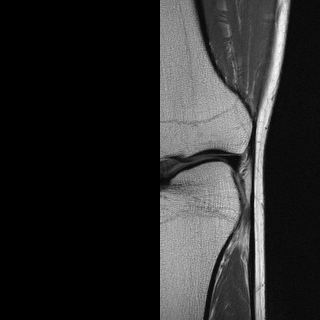
\includegraphics[frame, width=3cm]{../scripts/parallel-mri/ims1}};
		\node at (3.5, -3.2) {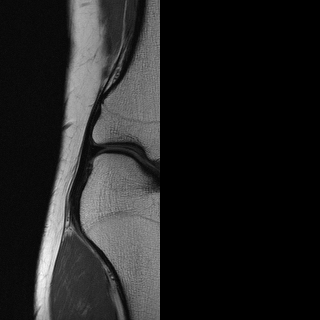
\includegraphics[frame, width=3cm]{../scripts/parallel-mri/ims2}};
		\node at (3.5, -5) {Coil images};

		\node at (7, 0) {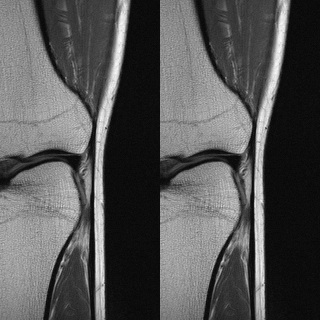
\includegraphics[frame, width=3cm]{../scripts/parallel-mri/image1}};
		\node at (7, -3.2) {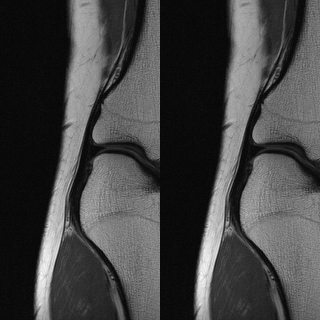
\includegraphics[frame, width=3cm]{../scripts/parallel-mri/image2}};
		\node at (7, -5) {Aliased reconstructions};

		\draw [maincolor, ultra thick] (7, 1.5) rectangle (8.5, -1.5);
		\draw [red!50!black, ultra thick] (7, -1.7) rectangle (5.5, -4.7);

		\begin{scope}[yshift=-1.6cm]
			\node at (10.5, 0) {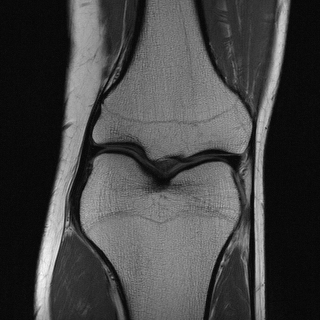
\includegraphics[frame, width=3cm]{../scripts/parallel-mri/reco}};
			\draw [maincolor, ultra thick] (10.5, 1.5) rectangle (12, -1.5);
			\draw [red!50!black, ultra thick] (10.5, 1.5) rectangle (9, -1.5);
			\draw [maincolor, ultra thick, dashed, dash phase=3pt] (10.5, 1.5) rectangle (12, -1.5);
			\draw [red!50!black, ultra thick, dashed] (10.5, 1.5) rectangle (9, -1.5);
			\node at (10.5, -1.8) {Reconstruction};
		\end{scope}
		\node at (14, -3.2) {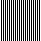
\includegraphics[frame, width=3cm]{../scripts/parallel-mri/mask}};
		\node at (14, -5) {Frequency selection};
		\node at (14, 0) {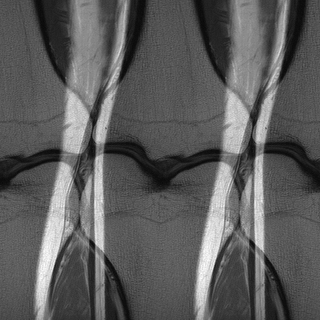
\includegraphics[frame, width=3cm]{../scripts/parallel-mri/aliased}};
		\node at (14, 1.8) {Naive reconstruction};
	\end{tikzpicture}
	\caption[The idea behind parallel imaging illustrated by an idealized example]{%
		The fundamental idea behind \gls{pils} algorithm~\cite{griswold_partially_2000} in an idealized case:
		The first column shows idealized coil sensitivities, each covering half of the measured area.
		The second column shows the underlying signal as seen by the coils; the third column are the per-coil naive reconstructions where the backfolding does not overlap the image.
		By taking the appropriate sections of each of the aliased coil images, the signal can be reconstructed exactly.
		On the right, the naive reconstruction with typical back-folding artifacts due to the frequency selection on the bottom is shown.
	}%
	\label{fig:pils}
\end{figure*}
However, the restriction to non-overlapping coil sensitivities and the required adaptation to the frequency selection renders the algorithm impractical.

The \gls{sense} algorithm due to Pruessmann et al.~\cite{pruessmann} extends this idea to arbitrary coil sensitivities and frequency selections.
Reconstructions are calculated by a linear weighting of the aliased coil images, where the weights are derived from the coil sensitivities.
Knowledge of the coil sensitivities necessitates a calibration scan in addition to the examination, and the speed-up is limited with classical linear reconstruction techniques due to noise amplification in regions where the sensitivities have significant overlap~\cite{Blaimer2004,pruessmann,Robson2008}.
The overlap is often characterized by the \enquote{geometry factor} or \( g \)-factor in the literature\cite{Robson2008}.

\Gls{pils} and \gls{sense} reconstruct the image from the aliased coil images.
In contrast to this are \gls{smash}~\cite{sodickson_simultaneous_1997} (more specifically, AUTO-SMASH~\cite{Jakob1998}) and \gls{grappa}~\cite{griswold_generalized_2002}.
These techniques reconstruct missing frequency data prior to Fourier inversion with the help of autocalibration data, which are typically low-frequency data in the center of the Fourier space.

In the intersection of these methods lies the popular ESPIRiT due to Uecker at al.~\cite{uecker_espirit_13}.
They demonstrated that coil sensitivities used in image domain approaches can be derived from autocalibration data used in frequency domain approaches.
Today, \gls{mri} reconstruction works typically use ESPIRiT to estimate coil sensitivities from autocalibration data~\cite{Aggarwal2019,darestani2021measuring,hammernik_learning_2017,jalal_robust_comporessed_2021,luo_bayesian_2023,zhu_image_2018}.
However, this explicit modeling of the coil sensitivities from autocalibration data has the drawbacks of prolonged scanning time and misalignment artifacts~\cite{Knoll2011,Ying2007}.
Additionally, most of the previous works assume a Cartesian frequency selection with measurements on a Cartesian grid,\footnote{%
	Acquiring frequencies off of the Cartesian grid is often called \emph{non-uniform} Fourier sampling.
} although radial, spiral or random sampling can be advantageous in different situations~\cite{lustid_compressed_2007,lustig2005faster,uecker_image_2008}.

To overcome the limitations of previous approaches, Bauer and Kannengiesser \cite{bauer_efficient_2007} propose to jointly estimate the image with the coil sensitivities.
Treating both as unknowns makes the reconstruction problem nonlinear; this is outlined later in~\cref{ssec:mri}.
We refer to the general principle as \emph{joint nonlinear inversion}.
They solve the joint nonlinear inversion using the iteratively regularized Gauss Newton method without any regularizers on the image or the coil sensitivities.
They treat the image and the coil sensitivities equally and do not resolve the ambiguity discussed in~\cref{ssec:mri} and consequently observe that the reconstruction is extremely sensitive to initialization, choice of regularization, and number of iterations of the algorithm.

Ying and Sheng independently proposed joint nonlinear inversion in~\cite{Ying2007} and resolve the ambiguity between the coil sensitivities and the image by observing that the coil sensitivities are \emph{much smoother than the image}.
They explicitly parametrize the coil sensitivities with low-order polynomials and solved the inversion using alternating minimization.
Uecker et al.~\cite{uecker_image_2008} built on this work but revisit the iteratively regularized Gauss Newton algorithm with smoothness of the coil sensitivities enforced through appropriate Sobolev norm penalties.
This approach was extended to include classic variational penalties on the image by Knoll et al.~\cite{Knoll2011} who report improved quantitative results using \gls{tv} and second-order \gls{tgv} regularization.

The work of Knoll et al.~\cite{Knoll2011} highlights the flexibility of formulating reconstruction as a nonlinear inverse problem.
Specifically, it accounts for smoothness penalties on coil sensitivities and sophisticated image regularization.
It is also not tied to Cartesian frequency selection and can account for nonuniform sampling.
However, their algorithm requires choosing multiple regularization parameters at each step and involves nontrivial subproblems to account for the variational penalties.

Our approach builds on the work of Knoll et al.~\cite{Knoll2011} but differs as follows:
Instead of handcrafted regularizers, we use modern generative learning techniques to learn an expressive regularizer from data, which leads to state-of-the-art reconstructions.
We enforce smoothness of the coil sensitivities quadratic gradient penalization gradient which simultaneously resolves ambiguities.
Instead of the iteratively regularized Gauss-Newton algorithm with non-trivial sub-problems, we employ the \gls{ipalm} algorithm~\cite{pock_inertial_2016} (\cref{alg:ipalm}) for optimization, ensuring convergence and requiring tuning of only two parameters (see~\cref{ssec:mri}).
Our reconstruction algorithm is sketched in~\cref{fig:reco} and takes about \qty{5}{\second} on consumer hardware.

For completeness, we mention that the end-to-end variational network of~\cite{sriram_endtoend_2020} also estimates the sensitivities jointly with the image.
However, their approach learns a mapping from frequency-space to image-space \emph{discriminatively}, using the estimated coil sensitivities to enforce data fidelity.
Thus, the network only works well with a particular frequency selection and coil configuration.
In contrast, we learn image features \emph{generatively} and impose handcrafted regularity onto the coil sensitivities.
\subsection{Related work}
\label{ssec:related work}
In this section we review related work on data-driven \gls{mri} reconstruction, focusing on methods similar to our proposed approach.
For a broader overview of data-driven \gls{mri} reconstruction, refer to~\cite{Zeng2021}.
Antun et al.~\cite{Antun2020} provide a comprehensive overview of the potential risks of using modern techniques for medical image reconstruction.

Guan at al.~\cite{Guan_energy_2022} explored learning a deep neural regularizer for \gls{mri} simultaneously to our work.
Unlike our approach but similar to the diffusion-based approaches discussed below, they apply their regularizer to the individual coil images in the reconstruction algorithm, requiring multiple evaluations of the gradient of the regularizer per iteration.
In addition, they estimate the sensitivity maps via ESPIRiT.\footnote{%
	Their exact reconstruction algorithm is unclear from their exposition.
}
In contrast, our joint nonlinear inversion algorithm eliminated the need for offline sensitivity estimation and requires only one gradient evaluation per iteration.

The authors extended their work in~\cite{tu_collaborative_2023} by learning an \gls{ebm} in image and frequency domain.
This eliminates the need for sensitivity estimation but requires training two independent networks that need to be balanced at inference time.
Additionally, the frequency-domain \gls{ebm} requires fully-sampled reference data, which is scarcely available.
Our method only requires reference DICOM (magnitude) images to train one regularizer.

Diffusion models are closely related to deep neural regularizers.
As discussed in~\cref{chap:pogmdm}, the score of a diffusion model \enquote{at time \num{0}} and the gradient of our regularizer model the same object:
The gradient of the negative log-prior.
Solving inverse problems with diffusion models is computationally demanding as it requires solving a \gls{sde} with high accuracy, typically requiring thousand of gradient evaluations~\cite{chung_scoremri_2022}.
Additionally, it is not clear how to optimally incorporate data-fidelity into the \gls{sde}.
Proposed solutions include data projection~\cite{song2022solving}, annealed Langevin dynamics~\cite{jalal_robust_comporessed_2021} and diffusion posterior sampling~\cite{chung2023diffusion}.
These methods require parameter tuning, in some cases at each step of the reverse diffusion~\cite{jalal_robust_comporessed_2021,chung2023diffusion}.
Feng at al.~\cite{feng2023scorebased} argue that none of these methods generate samples from the true posterior distribution and propose augmenting the score models with normalizing flows.
While their inference algorithm is parameter-free, the approach is opaque due to the introduction of the normalizing flow and is still computationally demanding.

Deep neural regularizers enjoy a natural probabilistic interpretation through Bayes theorem as discussed in~\cref{sec:variation methods and bayes theorem}.
\Gls{map} inference does not require solving an \gls{sde} and can be achieved by efficient through efficient optimization algorithms.
Access to the function value (not just the gradient) allows practical applications like inspecting the regularization landscape (see~\cref{fig:mri sampling}) and using backtracking in optimization algorithms~\cite{pock_inertial_2016}.%

Works by Luo et al.~\cite{luo_bayesian_2023} and Jalal et al.~\cite{jalal_robust_comporessed_2021} tackle parallel imaging by offline sensitivity estimation, which has drawbacks outlined in~\cref{ssec:parallel imaging intro}.
Chung et al.~\cite{chung_scoremri_2022} propose reconstructing individual coil images using a model trained solely on \gls{rss} reconstructions.
While the results are impressive, the computational cost depends on the number of coils and the authors report reconstruction times of up to \qty{10}{\minute}.
In our joint nonlinear inversion algorithm, the network's gradient is only evaluated once per iteration, regardless of the number of coils.
Imposing spatial regularity on the coils is extremely fast, requiring very few fast Fourier transforms at each iteration (see~\cref{ssec:mri}).

Finally, our generative approach has a practical benefit in the context of \gls{mri} reconstruction:
although we require \emph{reconstructions} from fully sampled data for training, it does not require fully sampled reference \emph{data}.
This distinction is important because reconstructions are more readily available in hospitals picture archiving and communication systems~\cite{zbontar_fastmri_2018}.
Constructing synthetic fully-sampled data from reference reconstructions is challenging due to the non-trivial interaction between coil sensitivities and the signal.
Most popular data-driven reconstruction algorithms like the end-to-end \gls{vn}~\cite{sriram_endtoend_2020}, AUTOMAP~\cite{zhu_image_2018}, and dual-domain approaches~\cite{tu_collaborative_2023,zhou2020dudornet} require image-data pairs for training.
Data-driven methods that need reference images include \glspl{gan}~\cite{Narnhofer2019}.
\Glspl{gan} suffer from the range-dilemma~\cite{bora_compressed_2017}, and authors have proposed to optimize the parameters of the \gls{gan} at inference time~\cite{Narnhofer2019}, effectively turning them into deep image priors~\cite{ulyanov_dip_2018}.
Deep image priors are challenging to optimize and don't offer a natural probabilistic interpretation.
\section{The pitfalls of discriminative signal recovery}%
\label{sec:discriminative pitfalls}
The classical way to utilizing deep learning methods in inverse problems involves learning a map from the data to the reconstruction \emph{discriminatively}.
However, this approach has significant drawbacks, particularly in medical imaging.
In this section we outline these drawbacks with a striking example.

The setup that we consider is as follows:\footnote{%
	We keep the setup general and don't specify any dimensionality or specific forward operator, \( A \), here.
}
We assume the signal to be reconstructed is an instance of a random variable \( X \) with density \( \DensityFunctionX \).
The data is summarized by a random variable related to the signals via
\begin{equation}
	Y = AX + N,
	\label{eq:relationship}
\end{equation}
where \( A \) is a linear operator with appropriate dimensions and \( N \) is Gaussian noise with known variance.
Thus, the signal and the data form a joint distribution \( p_{X\times Y} \) with the relationship between \( X \) and \( Y \) given by~\cref{eq:relationship}.

The discriminative approach in data-driven reconstruction methods involves a parametrized map \( f(\argm, \theta) \) that takes an instance of \( Y \) and outputs an estimation of \( X \).
The optimal parameters of the map are identified via the optimization problem
\begin{equation}
	\argmin_{\theta} \Expectation_{(X, Y) \sim p_{X\times Y}} \bigl[ l(f(Y, \theta), X) \bigr],
\end{equation}
where \( l \) is a loss function comparing the reconstruction \( f(y, \theta) \) with the reference signal \( x \).\footnote{Here, the lower case variables are instantiations of the corresponding random variables.}
Common loss functions include the negative \gls{ssim} (\cref{def:ssim}), and the two-norm or the one-norm of the difference.
This paradigm is extremely popular and includes pre-processing approaches~\cite{han_k-space_2020}, post-processing approaches~\cite{zbontar_fastmri_2018}, learned iterative networks~\cite{hammernik_learning_2017}, and AUTOMAP~\cite{zhu_image_2018}.

To emphasize the drawback of this approach, we consider the setup and baseline model from the original fastMRI publication~\cite{zbontar_fastmri_2018}.
Here, \( X \) is a random variable in \( \R^{\numproduct{320x320}} \) and \( \map{A = \Mask_{K}\Fourier}{\numproduct{320x320}}{\C^{\num{320}\times k}} \) is the Fourier transformation \( F \) followed by a Cartesian frequency selection, selecting \( k \in \mathbb{N} \) lines and \qty{8}{\percent} autocalibration lines, encoded in \( \Mask_{k} \);
this frequency selection operator is exemplified in the second column of~\cref{fig:simulation study masks}.
The map \( \map{f_k}{\C^{\num{320}\times k}}{\R^{\numproduct{320x320}}} \) is given by
\begin{equation}
	f_k(\argm, \theta) = \mathrm{UNet}(\argm, \theta) \circ \abs{} \circ \Adjoint{\Fourier}\Adjoint{\Mask_{k}}
\end{equation}
where \( \abs{} \) is the complex modulus acting element-wise on its argument and \( \mathrm{UNet}(\argm, \theta) : \R^{\numproduct{320x320}} \to \R^{\numproduct{320x320}} \) is a parametrized UNet.
This is a post-processing approach refining the zero-filling reconstruction with a learned UNet.
In the training, \( l \) is the one-norm and  \( k = \num{80} \) and the acceleration is \num{4}.

Let \( x \) be an image from the reference distribution, and let \( \Data_{k} = A_{k}x + n \) with n Gaussian noise.
\( k \in \mathbb{N} \) indicates the number of frequency lines that are available in the data.
For instance, when \( k = \num{320} \) the frequency space is completely filled.
\Cref{fig:unet kspace ablation} shows the \gls{psnr} of the reconstruction \( f_k(\Data_k, \theta) \) as \( k \) varies.
Notably, we observe that the \gls{psnr} decreases as \( k \) increases after around \( k = \num{140} \).
The reconstruction of the discriminative reconstruction network \emph{becomes worse as more data become available}.
\begin{figure*}
	\centering
	\begin{tikzpicture}[
		font=\footnotesize,
		rect annotation/.style={thick, fill, rectangle, inner sep=0.7mm},
	]
		\begin{axis}[
			xlabel={Available frequency lines},
			xticklabel={\pgfmathparse{\tick/320*100}\qty[round-mode=places,round-precision=0]{\pgfmathresult}{\percent}},
			ylabel={\gls{psnr} in \si{\decibel}},
			height=6cm, width=13cm,
			legend style={at={(1.06,.5)},anchor=west, draw=none},
			legend cell align={left},
		]
			\addplot [thick, black] table[col sep=comma, x=lines, y=naive]{chapters/deep-neural-regularizers/scripts/unet-kspace-ablation/psnr.csv};%
			\node (zero027) [rect annotation, black] at (axis cs:26, 22.26) {};
			\node (zero084) [rect annotation, black] at (axis cs:84, 22.96) {};
			\node (zero319) [rect annotation, black] at (axis cs:319, 46.14) {};

			\addplot [thick, red!50!black] table[col sep=comma, x=lines, y=unet]{chapters/deep-neural-regularizers/scripts/unet-kspace-ablation/psnr.csv};%
			\node (unet027) [rect annotation, red!50!black] at (axis cs:26, 25.63) {};
			\node (unet084) [rect annotation, red!50!black] at (axis cs:84, 32.02) {};
			\node (unet319) [rect annotation, red!50!black] at (axis cs:319, 29.03) {};

			\addplot [thick, maincolor] table[col sep=comma, x=lines, y=ours]{chapters/deep-neural-regularizers/scripts/unet-kspace-ablation/psnr.csv};%
			\node (ours027) [rect annotation, maincolor] at (axis cs:26, 25.44) {};
			\node (ours084) [rect annotation, maincolor] at (axis cs:84, 33.86) {};
			\node (ours319) [rect annotation, maincolor] at (axis cs:319, 46.67) {};
			\legend{Naive,Discriminative,Generative}
		\end{axis}
		\begin{scope}[xshift=1.5cm, yshift=-12.4cm]
			\foreach \offset/\kkappa in {0/027, 4.4/084, 8.8/319}
			{
				\node (\kkappa) [fill=maincolor, rectangle, inner sep=1mm] at (\offset-0.6, 0) {\includegraphics[rotate=180,width=4cm]{chapters/deep-neural-regularizers/scripts/unet-kspace-ablation/recos/ours/\kkappa}};
			}
		\end{scope}
		\begin{scope}[xshift=1.5cm, yshift=-8cm]
			\foreach \offset/\kkappa in {0/027, 4.4/084, 8.8/319}
			{
				\node (\kkappa) [fill=red!50!black, rectangle, inner sep=1mm] at (\offset-0.6, 0) {\includegraphics[rotate=180,width=4cm]{chapters/deep-neural-regularizers/scripts/unet-kspace-ablation/recos/unet/\kkappa}};
			}
			\node at (13.2-.7, 0) {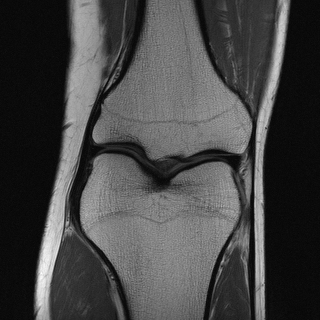
\includegraphics[rotate=180,width=4cm]{chapters/deep-neural-regularizers/scripts/unet-kspace-ablation/reference}};
			\node at (13.2-.6, 2.3) {Reference};
		\end{scope}
		\begin{scope}[xshift=1.5cm, yshift=-3.6cm]
			\foreach \offset/\kkappa in {0/027, 4.4/084, 8.8/319}
			{
				\node (\kkappa) [fill=black, rectangle, inner sep=1mm] at (\offset-0.6, 0) {\includegraphics[rotate=180,width=4cm]{chapters/deep-neural-regularizers/scripts/unet-kspace-ablation/recos/naive/\kkappa}};
				\draw [thick, black] (zero\kkappa.south) -- (\kkappa.north);
			}
		\end{scope}
	\end{tikzpicture}
	\caption[Discriminative signal recovery gets worse as more data becomes available]{%
		The signal recovered by the discriminative method deteriorates as more frequency lines become available:
		The reconstructions become overly sharp with accentuated details; when all data are available (\num{320} lines), the reconstruction is \qty{3.46}{\decibel} worse in \gls{psnr} than the reconstruction using \num{80} available frequency lines, which corresponds to the training setup.
		In contrast, due to the separation of likelihood and prior, the reconstruction of the generative approach improves with the availability of the data.
	}%
	\label{fig:unet kspace ablation}
\end{figure*}
\begin{sidefigure}
	\begin{tikzpicture}
		\node [inner sep=0, outer sep=0] at (0, 0) {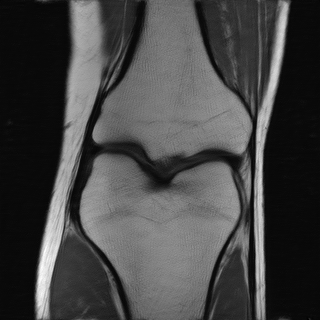
\includegraphics[rotate=180,width=4cm]{chapters/deep-neural-regularizers/scripts/unet-kspace-ablation/recos/radial}};
		\draw [white, -latex, ultra thick] (-.8, -1.3) -- ++(-.4, -.4);
	\end{tikzpicture}
	\caption[Reconstruction with radial frequency selection]{Reconstruction with radial frequency selection; the white arrow indicates obvious artifacts.}
	\label{fig:radial reco}
\end{sidefigure}
This is \emph{not} an out-of-distribution application of the reconstruction network:
The underlying signal \emph{is} drawn from the reference distribution \( \DensityFunctionX \), but we slightly change its relationship with the data \( \Data_k \).

While the decrease in \gls{psnr} is significant, the resulting reconstruction remains artifact-free when using Cartesian frequency selection.
However, switching to a radial frequency selection leads to reconstructions with obvious artifacts. 
The reconstruction in \cref{fig:radial reco} suggests that the network cannot distinguish between anatomical features and artifacts in the zero-filled reconstruction.
This issue can even occur with Cartesian frequency selection (see \cref{fig:simulation study}).

The major drawback of discriminative reconstruction methods is their performance deterioration when the acquisition operator changes, even when the underlying reference distribution remains unchanged.
This is due to the acquisition operator being integrated in the training setup, causing the learned components to entangle features of the reference data and characteristics of the acquisition operator.

Despite this drawback, data-driven reconstruction methods offer significant benefits when the data matches the training setup, outperforming hand-crafted regularizers.
In the remainder of this chapter, we explore how modern generative learning methods can be used to learn the reference distribution.
We adopt a Bayesian approach, separating the likelihood (which uses the acquisition operator) from the prior assumptions on the reference distribution.
We learn the latter using generative learning methods and utilize the learned model in a Bayesian variational reconstruction framework.
\section{Methods}%
\label{sec:methods}
In this section, we first detail the neural network architecture used as the regularizer.
Then, we discuss how the parameters of this regularizer can be learned from the reference distribution.
To use the regularizer in a joint nonlinear inversion framework, we derive an algorithm based on \gls{ipalm} that enforces nonnegativity of the spin density and spatial regularity of the coil sensitivities.
\subsection{Network architecture}%
\label{ssec:network architecture}
Typical regularizers used in imaging applications are of the ridge-type, as defined in~\cref{eq:ridge regularizers}.
These regularizers apply potentials to the responses of linear filters, summing over all filters and pixels.
This structure makes the regularizers translation invariant, which is desired in natural image reconstruction where the probability of a feature is independent of the spatial location.\footnote{This class of images is often referred to as texture-like.}
However, this is not the case for for the highly structures \gls{mri} images of the human knee where specific structures like vertically aligned bones surrounded by muscle- and fat tissue are expected.
In addition, these types of images usually come with nonlocal dependencies:
If a large amount of fat tissue is observed medially from the bone, usually a large amount of fat tissue is present laterally, see the example in \cref{fig:translation invariance}.
Classical regularizes are limited in their ability to resolve these large scale dependencies.

Ridge-type regularizers are also often preferred due to their interpretability:
Filters and corresponding potentials can be visualized, showing experts which structures are enhanced or diminished.
The architecture that we will now describe can not be interpreted in this way.
However, in~\cref{ssec:data independent analysis} we will provide an alternative way of visualizing preferred structures by means of drawing samples from the Gibbs distribution.
\begin{figure*}
	\begin{tikzpicture}
		\foreach [count=\imc] \impath/\annotation in {texture-gray/Texture, natural/Natural image, knee-mri/Knee \gls{mri}}
		{
			\node at (5.5*\imc, 0) {\includegraphics[width=5cm]{translation-invariance/\impath}};
			\draw [thick, maincolor] (5.5*\imc-2, 1.2) rectangle ++(1, 1) node [below right, maincolor] {\Large 1};
			\draw [thick, maincolor] (5.5*\imc+1, -1) rectangle ++(1, 1) node [below right, maincolor] {\Large 2};
			\node at (5.5*\imc, 2.8) {\annotation};
		}
	\end{tikzpicture}
	\caption[Translation (in-)variance and (non-)local dependencies in images]{%
		\tikzexternaldisable%
		Translation (in)variance and (non)local dependencies in images:
		In the texture-like image on the left (\texttt{matted\textunderscore{}0166.jpg} from the describable textures dataset~\cite{cimpoi14describing}), the probability of a feature does not depend on the spatial location.
		This is also a common assumption for natural images as the one in the middle (\texttt{103070.jpg} from \gls{bsds}~\cite{martin_database_2001}), since the image we see is a (more or less) arbitrary crop of the infinitely extending scene.
		On the contrary, for the knee image on the right (the central slice of \texttt{file1001057.h5} from the fastMRI knee dataset~\cite{zbontar_fastmri_2018}), we always see the femur on top of the tibia, which are both surrounded by muscle- and fat tissue.
		In addition, knee \gls{mri} images carry nonlocal dependencies:
		Since there is very little fat tissue medially (e.g.\ %
			\protect\tikz[baseline=-\the\dimexpr\fontdimen22\textfont2\relax]\protect\draw [thick, maincolor] (-.15, -.15) rectangle ++(.3, .3) node [below right, maincolor] {1};%
		), we also expect very little fat tissue laterally (e.g.\ %
			\protect\tikz[baseline=-\the\dimexpr\fontdimen22\textfont2\relax]\protect\draw [thick, maincolor] (-.15, -.15) rectangle ++(.3, .3) node [below right, maincolor] {2};%
		).
		\tikzexternalenable%
	}%
	\label{fig:translation invariance}
\end{figure*}

In this chapter, we depart from the ridge-type architecture, opting for a more general architecture that is \emph{not} translation invariant and \emph{can} resolve nonlocal dependencies.
We model the regularizer \( \map{R(\argm, \theta)}{\ImgDim}{\R} \) as a cascade of convolutional layers with leaky rectified linear unit activation functions.
The parameters \( \theta \) of the regularizer are made explicit in the second argument; they are detailed below.

Formally, the regularizer has the structure
\begin{equation}
	R(\argm, \theta) = \abs{} \circ W_{l+\num{1}} \circ L_l \circ L_{l-\num{1}} \circ \ldots \circ L_{\num{2}} \circ L_{\num{1}}.
	\label{eq:deep neural regularizer architecture}
\end{equation}
All \( l \) layers \( L_{\num{1}}, L_{\num{2}}, \dotsc, L_l \) follow the structure
\begin{equation}
	\begin{aligned}
		\map{L_i}{\R^{n_i \times n_i \times c_i}&}{\R^{n_{i + \num{1}} \times n_{i + \num{1}} \times c_{i + \num{1}}}},\\
		x &\mapsto \relu(\widetilde{W}_i \relu(W_i x)).
	\end{aligned}
\end{equation}
Here, leaky rectified linear unit activation function \( \relu \colon x \mapsto \max\{ \gamma x, x \} \) is applied point-wise and has a leakage parameter \( \gamma > \num{0} \).
The linear operator \( \map{W_i}{\R^{n_i \times n_i \times c_{i}}}{\R^{n_i \times n_i \times c_{i}}} \) encodes\footnote{%
	In the special case \( i = \num{1} \), \( \map{W_{\num{1}}}{\ImgDim}{\R^{\Height \times \Width \times c_{\num{1}}}} \).
	\label{foot:special handling of first layer}
} a convolution with a \numproduct{3x3} kernel with zero-boundary conditions, while the linear operator \( \map{\widetilde{W}_i}{\R^{n_i \times n_i \times c_{i}}}{\R^{n_{i + \num{1}} \times n_{i + \num{1}} \times c_{i+\num{1}}}} \) encodes a \emph{strided} convolution with stride \num{2}, reducing the feature map dimensions progressively.
Thus, \( n_{i + \num{1}} = n_i / \num{2} \) and \( n_{\num{1}} = n \).\footnote{%
	In our setting, this always results in a natural number. We discuss the choice of the number of layers \( l \) and the progression of the number of channels \( c_i \) in the implementation details.
}
The final linear operator \( \map{W_{l+\num{1}}}{\R^{n_{l+\num{1}} \times n_{l + \num{1}} \times c_{l + \num{1}}}}{\R} \) is a dense, fully learnable layer that maps to a real number, essentially encoding a learned weighted sum.
Denoting with \( w_i \in \R^{\num{3} \times \num{3} \times c_i \times c_i} \) and \( \widetilde{w}_i \in \R^{\num{3} \times \num{3} \times c_i \times c_{i + \num{1}}} \) the learnable filters of the convolution operators \( W_i \) and \( \widetilde{W}_i \) respectively, the learnable parameters in our model are \( \theta = {\{ w_l, \widetilde{w}_l \}}_{i=\num{1}}^l \cup \{ W_{l+1} \} \).

Unlike ridge-type architectures where feature map responses are summed, our model progressively downsamples the feature maps via learned convolutions and nonlinearities until they are reduced to a scalar via a learned weighted sum.
This regularizer is not translation invariant and  it can prefer certain structures in certain regions, accommodation nonlocal structure arrangements.

The architecture of our regularizer can also be motived by considering its gradient with respect to the input image.\footnote{%
	The network is not differentiable; the gradient can be understood either via a differentiable surrogate of the rectified linear unit or in the sense of the Clarke subdifferential~\cref{def:clarke subdifferential}.
}
To derive the gradient, we note that \( L_i = \relu \circ \widetilde{W}_i \circ \relu \circ W_i \) and denote the \emph{activations} \( \relu^\prime \) of the point-wise activation functions after the convolution operators \( W_i \) and \( \widetilde{W}_i \) as
\begin{equation}
	a_i(x) = \bigl(\relu^\prime \circ W_i \circ L_{i-1} \circ \ldots \circ L_{\num{1}}\bigr)(x)
\end{equation}
and
\begin{equation}
	\tilde{a}_i(x) = \bigl(\relu^\prime \circ \widetilde{W}_i \circ \relu \circ W_i \circ L_{i-1} \circ \ldots \circ L_{\num{1}}\bigr)(x).
\end{equation}
We denote the activation of the final fully connected layer as
\begin{equation}
	a_{l + 1}(x) = \bigl( \abs{}^\prime \circ W_{l+1} \circ L_l \circ \ldots \circ L_{\num{1}} \bigr)(x).
\end{equation}
Then, by backpropagation
\begin{equation}
	\begin{aligned}
		&(\Grad R(\argm, \theta))(x) = \\
		&\Adjoint{W_{\num{1}}} \bigl( a_{\num{1}}(x) \cdot \Adjoint{\widetilde{W}_{\num{1}}} \bigl( \ldots \bigl( \tilde{a}_{l-1}(x) \cdot \Adjoint{W_l} \bigl( a_l(x) \cdot \Adjoint{\widetilde{W}_{l}}\bigl(\tilde{a}_l(x) \cdot \Adjoint{W_{l+1}} a_{l+1}(x) \bigr) \bigr) \bigr) \ldots \bigr) \bigr)
	\end{aligned}
\end{equation}
which has the structure of a UNet.

The UNet architecture, introduced by Ronneberger et al.\ in 2015~\cite{ronneberger_unet_2015}, has gained immense popularity in many applications requiring maps from the signal space to itself.\footnote{%
	The output space can also be \enquote{slightly different}. This is the case for instance in dense labeling or segmentation.
}
The key idea behind UNet is to capture context in the contracting path (via consecutive strided convolutions) and subsequently retrieve details in the expanding path (via consecutive adjoint strided convolutions).
To ensure detailed recovery in the expanding path and avoid loss of information, UNet employs \emph{skip connections} that retrieve features from the layers in the contracting path.
This is typically realized by concatenating the feature maps.

In modeling the gradient of a probability density, UNet-type architectures have become the standard backbone for diffusion models.\footnote{%
	We discuss diffusion models in more detail in~\cref{chap:pogmdm}. The relationship between our approach and diffusion models is covered superficially in~\cref{ssec:related work}
}
Works include the seed papers on diffusion models~\cite{song_generative_2019,song2021scorebased} and recent works that utilize diffusion models to solve inverse problems~\cite{chung_scoremri_2022,jalal_robust_comporessed_2021,chung2023solving,chung2023diffusion}.
A common criticism of these models (that we also make in this chapter and in~\cref{chap:pogmdm}) is that these networks are in general not a gradient.
This issue was noted in the paper on sliced score matching~\cite[footnote 1 on page 4]{song2020sliced}, a precursor to diffusion model papers, where the authors argued that the lack of gradient property does not significantly impact practical applications.

In contrast, our approach naturally retrieves a UNet-type model as the gradient of our scalar function.
The expanding path in each layer uses the adjoint operators of the corresponding contracting path layer.
The skip connections are realized by scalar multiplication of the feature maps in the expanding path by the activation from the contracting path.
This structure is schematically illustrated in~\cref{fig:deep neural regularizer architecture}.
\begin{figure*}
	\def\convcolor{rgb:blue,4;red,1;green,4;black,3}
	\def\skipcolor{rgb:blue,4;red,1;green,1;black,3}
	\def\FcColor{rgb:blue,5;red,2.5;white,5}
	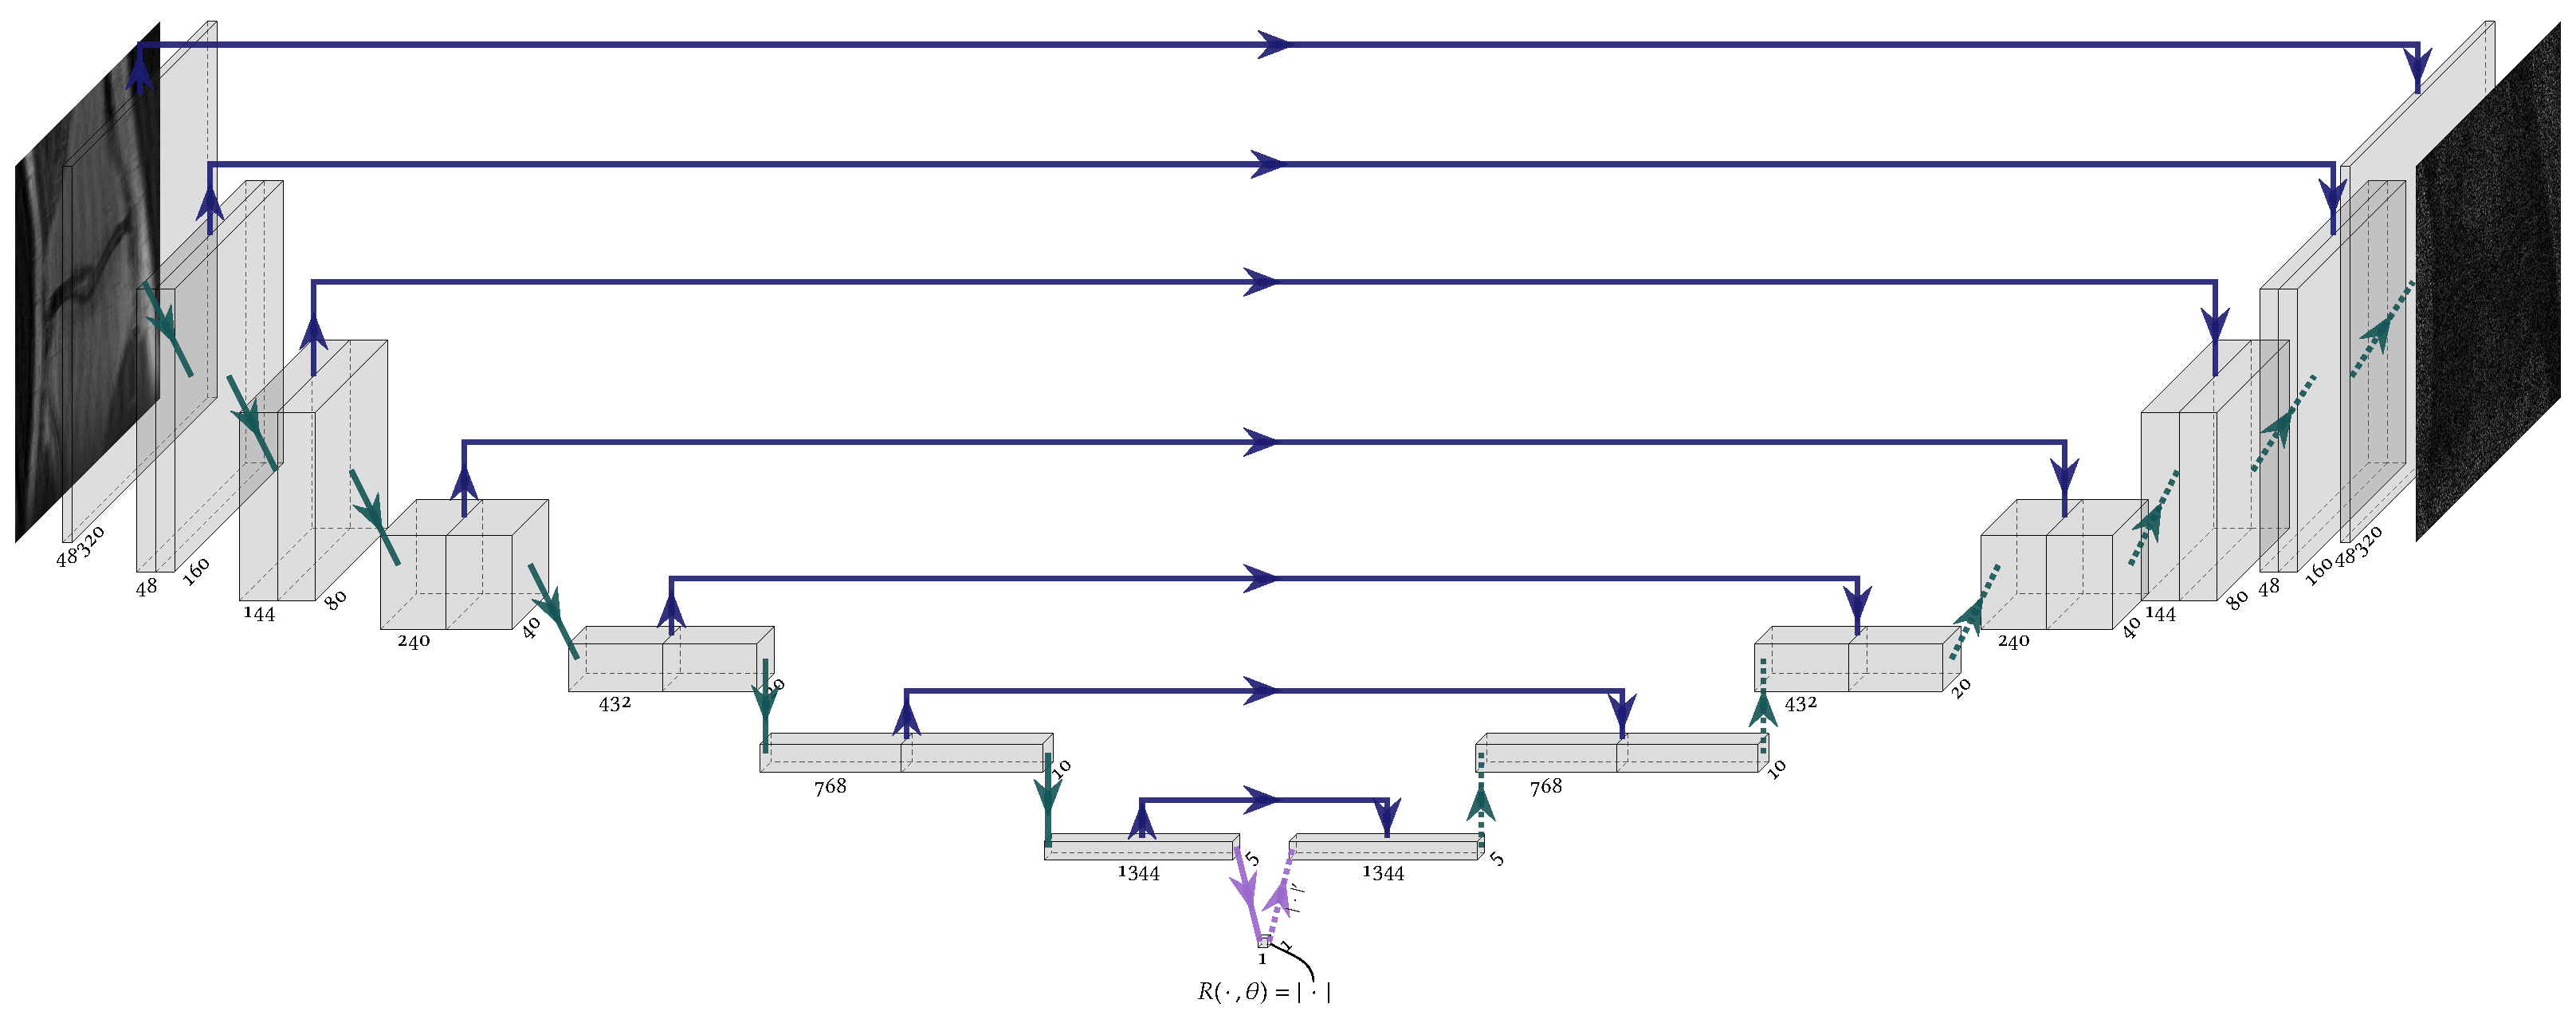
\includegraphics[width=\linewidth]{network/gradient}
	\caption[Schematic of the gradient of the regularizer: A UNet]{%
		\tikzexternaldisable%
		The gradient of the regularizer has a UNet structure.
		At the \( i \)-th layer, the symbol %
			\protect\tikz[baseline=-\the\dimexpr\fontdimen22\textfont2\relax]\protect\draw [thick,draw=\convcolor, -Stealth] (0, 0) -- ++(.5, 0); %
		is the map \( x \mapsto \relu(\widetilde{W}_ix) \), and %
			\protect\tikz[baseline=-\the\dimexpr\fontdimen22\textfont2\relax]\protect\draw [thick,draw=\convcolor, -Stealth, dashed] (0, 0) -- ++(.5, 0); %
		is the map \( x \mapsto \Adjoint{\widetilde{W}_i}x \); the convolutions with unit stride are between the gray blocks and (for the sake of simplicity) are not endowed with an arrow.
		The skip connection
			\protect\tikz[baseline=-\the\dimexpr\fontdimen22\textfont2\relax]\protect\draw [thick,draw=\skipcolor, -Stealth] (0, 0) -- ++(.5, 0); %
		is understood as the map \( x \mapsto \relu^\prime(x) \), the result of which pointwise multiplies the features in the expanding path.
		The function value of the network is given as the absolute value of the scalar-valued feature map at the bottom, which is computed via the learned weighed sum (the fully connected layer \( W_{l+1} \)) %
			\protect\tikz[baseline=-\the\dimexpr\fontdimen22\textfont2\relax]\protect\draw [thick,draw=\FcColor, -Stealth, dashed] (0, 0) -- ++(.5, 0);.
		The annotations show the size of the feature maps.
		The illustration is slightly simplified; we neither explicitly show the nonstrided convolutions (these would be arrows between the adjacent blocks) nor their corresponding skip connections.
		\tikzexternalenable%
	}%
	\label{fig:deep neural regularizer architecture}
\end{figure*}

While our approach imposes some restrictions compared to a classical UNet, it accurately models the gradient of the log-prior, as empirically demonstrated in \cref{fig:mri sampling deep neural regularizers}.
Moreover, our model allows for the computation of function values, not just gradients, while preserving classical symmetry properties of gradients.
In the next section, we discuss how to learn the parameters of the regularizer such that is accurately models the negative log-prior.
\subsection{Parameter identification}%
\label{ssec:methods ml}
In the strict Bayesian view of inverse problems that we adopt in this thesis, we assume that in any reconstruction problem, the underlying signal is a realization of a random variable \( X \) with density \( \DensityFunctionX \).
In this chapter, the random variable has values in \( \ImgDim \) and represents the magnitude of \gls{mri} scans of the human knee, see the details in \cref{ssec:details}.
In this view, the regularizer in the inverse problem models the negative log-prior, up to an additive constant.

Under mild conditions we can associate any regularizer \( R(\argm,\theta) \) with a density
\begin{equation}
	\hat{\DensityFunction}_{\RandomVariable}(x) = \frac{\exp\bigl(-R(x,\theta)\bigr)}{\int_{\ImgDim}\exp\bigl(-R(\xi, \theta)\bigr)\,\mathrm{d}\xi}.
	\label{eq:gibbs}
\end{equation}
When \( R(\argm, \theta) \) is of ridge-type, then this construction is called a \emph{Gibbs distribution}, see~\cite[theorem 1 and the two preceding definitions]{zhu_filters_1998} and~\cite[page 5]{geman_stochastic_1984}.
Modern literature extend this to more general functions, including neural networks, which can also induce a Gibbs distribution via the equation above~\cite[section 3.1]{nijkamp_shortrun_2019},~\cite[section 2.1]{nijkamp_anatomy_2019}.

\( R(\argm, \theta) \) admits a Gibbs density if it is bounded from below and grows \enquote{fast enough} radially, such that \( \int_{\ImgDim}\exp\bigl(-R(\xi, \theta)\bigr)\,\mathrm{d}\xi < \infty \).
We ensure boundedness from below by using an absolute value activation in the last layer.
The growth condition can be achieved by adding a small quadratic term to the regularizer\footnote{%
	This is also a popular strategy to assign a proper distributions to ridge-type regularizers, see e.g.~\cite[eq. (1)]{schmidt_generative_2010} and~\cite[eq. (6)]{weiss_model_2007}.
} but in practice this is unnecessary.

Identifying the optimal parameters of the regularizer becomes a problem of density fitting, and we adopt the popular approach of minimizing the Kullback-Leibler divergence from \( \DensityFunctionX \) to \( \DensityFunctionXEstimation \).
The Kullback-Leibler divergence is popular due to the links to maximum likelihood and maximum entropy estimation.
Seminal papers that utilize it include~\cite{hinton_training_2002,RoBl09,zhu_filters_1998}; it has been called the \enquote{standard} divergence by Teh, Welling, Osindero and Hinton in~\cite{teh_energy_2003}.
The Kullback-Leibler divergence from \( \DensityFunctionX \) to \( \DensityFunctionXEstimation \) (see~\cref{def:kullback leibler divergence}) reads
\begin{equation}
	\KullbackLeibler{\DensityFunctionX}{\DensityFunctionXEstimation} = \int_{\ImgDim} \DensityFunctionX(x)\log\frac{\DensityFunctionX(x)}{\DensityFunctionXEstimation(x)}\,\mathrm{d}x.
	\label{eq:kullback leibler deep neural regularizers}
\end{equation}
As is common in the literature, we do not ensure that \( \DensityFunctionX \) is absolutely continuous (see~\cref{def:absolute continuity}) with respect to \( \DensityFunctionXEstimation \).
Even without guaranteeing this, we can \enquote{notationally} derive a learning objective that is useful in practice.

To derive the objective for parameter identification, we make the parametrization more explicit and write \( \DensityFunctionXEstimation \coloneqq \DensityFunctionXEstimation(\argm; \theta) \).
The minimization objective to identify the optimal parameters\footnote{%
	We discuss the set of admissible parameters \( \Theta \) in~\cref{ssec:details}.
} is
\begin{equation}
	\begin{aligned}
		&\argmin_{\theta \in \Theta}\,\KullbackLeibler{\DensityFunctionX}{\DensityFunctionXEstimation(\argm; \theta)} = \\
		&\argmin_{\theta \in \Theta} \int_{\ImgDim} \DensityFunctionX(x)\log\frac{\DensityFunctionX(x)}{\DensityFunctionXEstimation(x; \theta)}\,\mathrm{d}x = \\
		&\argmin_{\theta \in \Theta} \int_{\ImgDim} \DensityFunctionX(x) \bigl( - \log \DensityFunctionXEstimation(x; \theta)\bigr)\,\mathrm{d}x
	\end{aligned}
\end{equation}
where the last equality holds since the density of the reference distribution does not depend on the parameters.
Rewriting in terms of expectations (\cref{def:expectation}) reveals the celebrated maximum likelihood objective
\begin{equation}
	\argmin_{\theta \in \Theta} \Expectation_{X\sim p_X}\bigl[-\log \DensityFunctionXEstimation(X; \theta) \bigr].
\end{equation}
Inserting the Gibbs density~\cref{eq:gibbs} into the above yields
\begin{equation}
	\argmin_{\theta \in \Theta} \Expectation_{X\sim p_X}\bigl[ R(X, \theta) \bigr] + \log\int_{\ImgDim}\exp\bigl(-R(\xi, \theta)\bigr)\,\mathrm{d}\xi.
\end{equation}

We solve the parameter identification via first order algorithms and consequently find the gradient with respect to the parameters by the chain rule as
\begin{equation}
	\int_{\ImgDim}\frac{\exp\bigl(-R(x, \theta)\bigr)}{\int_{\ImgDim}\exp\bigl(-R(\xi, \theta)\bigr)\,\mathrm{d}\xi} \bigl(-\Grad_{\num{2}} R(x, \theta) \bigr)\,\mathrm{d}x = \Expectation_{X\sim\DensityFunctionXEstimation}\bigl[-\Grad_{\num{2}} R(X, \theta) \bigr].
\end{equation}
Thus, parameter identification amounts to finding
\begin{equation}
	\argmin_{\theta \in \Theta} \Expectation_{X\sim\DensityFunctionX} \bigl[ R(X, \theta) \bigr] -\Expectation_{X\sim\DensityFunctionXEstimation} \bigl[ R(X, \theta) \bigr].
	\label{eq:difference of expectations}
\end{equation}

This derivation has been used in the context of parameter identification of densities at least since the eighties~\cite{ackley1985learning}.
In some sense,~\cref{eq:difference of expectations} is the most general\footnote{%
	In the sense that it follows directly from maximum likelihood learning of the completely general family of Gibbs distributions with arbitrary potential.%
} way of fitting densities.
In the context of Boltzmann machines, it was termed the \emph{wake-sleep} algorithm~\cite{hinton1995wake} (the earliest reference we could find that mentions the word \enquote{sleep} in this context was~\cite{freund1991unsupervised}).
When the expectation over the Gibbs distribution is approximated via few-step \gls{mcmc} initialized with reference samples, the resulting algorithm is known as \emph{contrastive divergence}~\cite{hinton_training_2002}.

The primary challenge in~\cref{eq:difference of expectations} is computing the expectation over the Gibbs distribution \( \DensityFunctionXEstimation \).
In the context of Boltzmann machines, \emph{restricted} Boltzmann machines~\cite{rumelhart1986parallel} address this by restricting the architecture of the learned functions.
For data-driven regularizers in imaging, Schmidt, Gao, and Roth~\cite{schmidt_generative_2010} exploit the special structure of their regularizer and derive an efficient auxiliary variable Gibbs sampler to approximate the expectation.
Conversely, Weiss and Freeman~\cite{weiss_model_2007} focus on regularizers where the partition function is parameter independent, allowing them only to learn a rotation of predefined filters in a ridge-regularizer with Gaussian scale mixture potentials.
They develop an efficient expectation-maximization algorithm to learn the weights of the Gaussian scale mixture and the rotation.

The method we adopt in this work aligns more closely with the \gls{foe} work by Roth and Black~\cite{RoBl09} and recent literature on generative models~\cite{nijkamp_shortrun_2019,du_implicit_2019}.
Specifically, we resort to \gls{mcmc} algorithms to approximate the expectation.
Following~\cite{nijkamp_shortrun_2019,du_implicit_2019} we use the unadjusted Langevin algorithm shown in~\cref{alg:unadjusted langevin algorithm} to sample from the Gibbs distribution.
The algorithm's motivation, properties and detailed analyses are covered in~\cref{ssec:diffusion processes};
here, we recall is key properties and adapt the notation.

The unadjusted Langevin algorithm
\begin{equation}
	x^{k+\num{1}} = x^k + \tau \Grad \log \DensityFunctionXEstimation(x^k) + \sqrt{\num{2}\tau}z^k
	\label{eq:_ula}
\end{equation}
with \( x^{\num{0}} \) arbitrary and \( z^k \sim \NormalDistribution_{\num{0}, \Identity} \), results from an Euler-Maruyama discretization\footnote{%
	with equispaced discretization time points, separated by \( \tau > \num{0} \)
} of the continuous Langevin diffusion (\cref{eq:langevin diffusion}).
The continuous Langevin diffusion has invariant distribution \( \DensityFunctionXEstimation \) as shown in~\cref{th:convergence of langevin diffusion}.
Although the discretization introduces bias, Durmus, Moulines, and Pereyra~\cite{durmus_efficient_18} found that adding a Metropolis-Hastings correction step often worsens results in practice, so we exclude this step.

By inserting the Gibbs distribution in~\cref{eq:_ula},
\begin{equation}
	x^{k+1} = x^k - \tau \Grad R(x^k, \theta) + \sqrt{\num{2}\tau}z^k.
	\label{eq:ula regularizer}
\end{equation}
which simplifies to a \enquote{noisy} gradient descent\footnote{%
	Again we remark that our regularizer is not differentiable.
	The gradient here is understood as a Clarke subdifferential and we discuss works that deal with this setup in~\cref{ssec:diffusion processes}.
} on the regularizer since the normalization constant vanishes.

During learning, we run the unadjusted Langevin algorithm after every parameters update since parameter updates change the Gibbs distribution.
To make the learning algorithm  practical, it is crucial to minimize the required steps until the Markov chain (\cref{def:markov chain}) converges.
This can be achieved by an informed initialization:
Since parameter updates are usually small,\footnote{%
	This depends on the learning rate of the optimizer, but typically this is true.%
} the Gibbs distribution should remain similar between parameter updates.
Thus, \emph{samples} from the distribution prior to the update serve as good \emph{initializations} for the Markov chain post-update.
This algorithm due to Tieleman~\cite{tieleman_training_2008} is known as \emph{persistent contrastive divergence}.
We use this method to facilitate training our regularizer, with implementation details discussed in~\cref{ssec:details}.
\subsection{Reconstruction algorithm}%
\label{ssec:mri}
In this work we revisit joint nonlinear inversion for parallel \gls{mri} reconstruction.
This approach aims to estimate spatially varying coil sensitivities along with the image in a nonlinear inverse problem, thereby utilizing the available data optimally.
Detailed motivation for this is discussed in~\cref{ssec:related work};
here we outline our proposed algorithm and point again to the works of Bauer and Kannengiesser~\cite{bauer_efficient_2007}, Ying and Sheng~\cite{Ying2007} and Uecker, Hohage, Block, and Frahm~\cite{uecker_image_2008} which sparked this line of research.

We assume that the parallel \gls{mri} machine has \( c \in \mathbb{N} \) receiver coils that sense the spin density of the scanned object.
The sensitivities of the receiver coils are complex images \( \sigma_{\num{1}}, \sigma_{\num{2}}, \dotsc, \sigma_c \in \C^{m \times n} \) defined on the same grid as the image.
The measurement data are then \( c \) vectors \( \Data_{\num{1}}, \Data_{\num{2}}, \dotsc, \Data_c \in \C^f \) where \( f \in \mathbb{N} \) is the number of acquired frequencies.
We assume that these frequencies are grid-aligned, though nonuniform sampling is possible (see~\cite{Smith2018}).

The data relate to the underlying image via a discrete Fourier transform \( \map{\Fourier}{\C^{m \times n}}{\C^{m\times n}} \) and a binary diagonal operator \( \map{\Mask}{\C^{m \times n}}{\C^f} \) which picks the acquired frequencies.\footnote{
	The notation is chosen in analogy to~\cref{chap:regularizers}.
}
Thus, the spin density, coil sensitivities and data relate through\footnote{%
	Nonuniform sampling is easily realized by substituting \( \Mask\Fourier \) with the appropriate nonuniform Fourier transform.
	The remaining derivation carries over to this case.
}
\begin{equation}
	\begin{aligned}
		\Data_{\num{1}} &= \Mask\Fourier(\sigma_{\num{1}} \odot x) + \eta_{\num{1}},\\
		\Data_{\num{2}} &= \Mask\Fourier(\sigma_{\num{2}} \odot x) + \eta_{\num{2}},\\
			&\vdotswithin{=} \\
		\Data_c &= \Mask\Fourier(\sigma_c \odot x) + \eta_c,
	\end{aligned}
	\label{eq:data for parallel imaging}
\end{equation}
where \( \eta_{\num{1}}, \eta_{\num{2}}, \dotsc, \eta_c \in \C^f \) are coil-wise additive noise terms.

The data \( \Data_{\num{1}}, \Data_{\num{2}}, \dotsc, \Data_c \) have a \emph{nonlinear} relation to the estimation variables \( x, \sigma_{\num{1}}, \sigma_{\num{1}}, \dotsc, \sigma_c \).
The bilinear structure introduces ambiguity: 
multiplying the spin density with an arbitrary image \( w \in \C^{\Height \times \Width} \) and dividing the coil sensitivities by \( w \) yields the same solution: \( (\sigma_i \odot x) = \bigl((\sigma_i \oslash w) \odot (x \odot w) \bigr)\).
To resolve this, we regularize the image \( x \) and the coil sensitivities \( \sigma_{\num{1}}, \sigma_{\num{2}}, \dotsc, \sigma_c \).
We use the data-driven regularizer described in \cref{ssec:network architecture} for the image and classical quadratic gradient penalization for the coil sensitivities.

We formalize the nonlinear inversion problem as an optimization problem.
Let \( \Sigma = (\sigma_{\num{1}}, \sigma_{\num{2}}, \dotsc, \sigma_c) \in \C^{m \times n \times c} \).
Data consistency is ensured using a quadratic data fidelity
\begin{equation}
	\begin{aligned}
		\map{D}{\R^{m\times n} \times\C^{m\times n \times c}&}{\C^{m\times n \times c}} \\
		(x, \Sigma) &\mapsto \Half \sum_{i=\num{1}}^c \norm*{\Mask\Fourier(\sigma_i \odot x) - z_i}_{\num{2}}^{\num{2}}.
	\end{aligned}
\end{equation}
We regularize the image with our data-driven regularizer \( R(\argm, \theta) \) from \cref{ssec:network architecture} \footnote{%
	The algorithm that we derive does not explicitly require our data-driven regularizer;
	also classical regularizers such as the \gls{tv} can be used.
	The numerical results in~\cref{ssec:parallel imaging} use the \gls{tv} regularizer embedded in the algorithm.
} and explicitly enforce nonnegativity of the image during optimization.
To resolve the ambiguity in the bilinear form, we ensure that the coil sensitivities are sufficiently smooth by utilizing classical quadratic gradient penalization through
\begin{equation}
	\begin{aligned}
		\map{S}{\C^{m\times n \times c}&}{\R} \\
		\Sigma &\mapsto \Half \sum_{c=\num{1}}^{C} \big( \norm{\DiffOp_{\mathrm{D}} \mathfrak{Re}(\sigma_c)}_{\num{2}}^{\num{2}} + \norm*{\DiffOp_{\mathrm{D}} \mathfrak{Im}(\sigma_c)}_{\num{2}}^{\num{2}} \big),
	\end{aligned}
\end{equation}
where \( \map{\DiffOp_{\mathrm{D}}}{\R^{m\times n}}{\R^{m\times n \times \num{2}}} \) is a forward finite difference operator with Dirichlet boundary conditions:
\begin{equation}
	\begin{aligned}
		(\DiffOp_{\mathrm{D}} x)_{i, j, \num{1}} &= \begin{cases}
			x_{i + \num{1}, j} - x_{i, j} & \text{if}\ \num{1} \leq i < m, \\
			-x_{i, j} & \text{else},
		\end{cases}\\
			(\DiffOp_{\mathrm{D}} x)_{i, j, \num{2}} &= \begin{cases}
			x_{i,j + \num{1}} - x_{i,j} & \text{if}\ \num{1} \leq j < n, \\
			-x_{i, j} & \text{else}.
		\end{cases}
	\end{aligned}
\end{equation}
These conditions assume coil sensitivities are zero outside the image domain, reflecting physical reality.

Recovering the image \( x \) and coil sensitivities \( \sigma_{\num{1}}, \sigma_{\num{2}}, \dotsc, \sigma_c \) from the data \( \Data_{\num{1}}, \Data_{\num{2}} \dotsc, \Data_c \) amounts to finding
\begin{equation}
	\argmin_{x \in \R^{m \times n}, \Sigma \in \C^{m \times n \times c}} D(x, \Sigma) + \lambda R(x, \theta) + \IndicatorFunction{\R^{m\times n}_+}(x) + \mu S(\Sigma),
	\label{eq:joint inversion optimization problem}
\end{equation}
where \( \IndicatorFunction{\R^{m\times n}} \) is the indicator function (\cref{def:indicator function}) of the nonnegative orthant, and \( \lambda, \mu > \num{0} \) tune the influence of the image and the coil sensitivity regularization.

We now detail the algorithm that solves the optimization problem~\cref{eq:joint inversion optimization problem}.\footnote{%
	All gradients are understood in the \( \mathbb{C}\mathbb{R} \)-sense~\cite{kreutz_complex_2009}.%
}
Despite being nonconvex and nonsmooth, the problem has a favorable structure:
the smooth part has a Lipschitz continuous gradient in both variable blocks, and the proximal map for the nonsmooth functions can be efficiently computed.
For a fixed \( \Sigma \), the map \( x \mapsto D(x, \Sigma) + \lambda R(x, \theta) \) has a Lipschitz continuous gradient\footnote{%
	when \( \nabla R(\argm, \theta) \) is Lipschitz.
	This is the case when we utilize differentiable surrogates of the rectified linear activation.
}
\begin{equation}
	x \mapsto \sum_{i=\num{1}}^c \conj{\sigma_i} \odot (\Adjoint{\Fourier}\Adjoint{\Mask}(\Mask\Fourier(\sigma_i\odot x) - z_i)) + \lambda \Grad_{\num{1}} R(x, \theta).
\end{equation}
Analogously, for a fixed \( x \), the map\footnote{We include the term \( \lambda R(x, \theta) \) here to emphasize the structure.} \( \Sigma \mapsto D(x, \Sigma) + \lambda R(x, \theta) \) has a Lipschitz continuous gradient
\begin{equation}
	\Sigma \mapsto \begin{pmatrix}
		x \odot (\Adjoint{\Fourier}\Adjoint{\Mask}(\Mask\Fourier(\sigma_{\num{1}}\odot x) - z_i)) \\
		\vdotswithin{%
			x \odot (\Adjoint{\Fourier}\Adjoint{\Mask}(\Mask\Fourier(\sigma_i\odot x) - z_{\num{1}}))
		} \\
		x \odot (\Adjoint{\Fourier}\Adjoint{\Mask}(\Mask\Fourier(\sigma_c\odot x) - z_c)) \\
	\end{pmatrix}.
\end{equation}
The proximal maps (\cref{def:proximal operator}) for \( \IndicatorFunction{\R^{m\times n}} \) and \( \mu S \) are efficiently computed:
The proximal map of the indicator function of the nonnegative orthant, \( \map{\prox_{\IndicatorFunction{\R^{m\times n}}}}{\R^{m\times n}}{\R^{m\times n}} \), retrieves the positive part of its argument:
\begin{equation}
	\prox_{\IndicatorFunction{\R^{m\times n}}}(x) = \max(x, \num{0}).
\end{equation}
The proximal map of the quadratic gradient penalization, \( \map{\prox_{\IndicatorFunction{\R^{m\times n}}}}{\C^{m\times n \times c}}{\C^{m\times n \times c}} \) uses the discrete sine transform:
Denoting the imaginary unit with \( \hat{\imath} \coloneqq \sqrt{\num{-1}} \),
\begin{equation}
	\prox_{\mu S}(\Sigma) = \begin{pmatrix}
		Q_\mu(\mathfrak{Re}(\sigma_{\num{1}})) + \hat{\imath} Q_\mu(\mathfrak{Im}(\sigma_{\num{1}})) \\
		\vdotswithin{%
			Q_\mu(\mathfrak{Re}(\sigma_c)) + \hat{\imath} Q_\mu(\mathfrak{Im}(\sigma_c))
		} \\
		Q_\mu(\mathfrak{Re}(\sigma_c)) + \hat{\imath} Q_\mu(\mathfrak{Im}(\sigma_c))
	\end{pmatrix}.
\end{equation}
Here,
\begin{equation}
	\map{Q_\mu}{\R^{m\times n}}{\R^{m\times n}} \colon x \mapsto \Adjoint{\DiscreteSineTransform} \bigl(\DiscreteSineTransform(\mu x) \oslash (\xi + \mu) \bigr)
\end{equation}
uses the two-dimensional discrete sine transform \( \DiscreteSineTransform \), where \( \xi \) are the eigenvalues of the two-dimensional discrete Laplace operator\footnote{%
	This is essentially a fast Poisson solver, see~\cite[Chapter 19.4]{press_numerical_1992} for a more rigorous discussion.%
}
\begin{equation}
	\xi_{i, j} = \num{4} - \num{2} \bigl(\cos \frac{\pi i}{m} + \cos \frac{\pi j}{n} \bigr)
\end{equation}
We show the smoothing action of this proximal map in~\cref{fig:h1 smoothing}.
\begin{sidefigure}
	\centering
	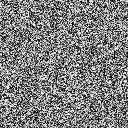
\includegraphics[width=\marginparwidth]{prox/input}\\
	\ \ \ \ \ \ \ \ \ \( \downarrow \prox_{S} \)\\
	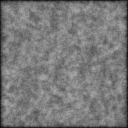
\includegraphics[width=\marginparwidth]{prox/proxed}
	\caption[Smoothing via proximal map of quadratic gradient norm]{%
		The smoothing action of the proximal operator with respect to quadratic gradient penalization with Dirichlet boundary conditions.
	}%
	\label{fig:h1 smoothing}
\end{sidefigure}
There, in the image on top the real and imaginary part of each pixel is drawn uniformly in \( \interval{\num{0}}{\num{1}} \), we set \( \mu = \num{3} \) and only show the real part.
The image is significantly smoother and smoothly approaches zero at the boundaries.

The structure outlined above is exploited in the \gls{ipalm} algorithm by Pock and Sabach~\cite{pock_inertial_2016}.
In the iterations, we use backtracking to estimate the Lipschitz constants; the algorithm is summarized in~\cref{alg:ipalm for mri generic verison}.
As already pointed out, this algorithm can use any image regularizer.
For our experiments we tweak it for optimal performance under our particular setup with the details discussed in~\cref{ssec:details}.
A sketch of the reconstruction algorithm is shown in~\cref{fig:reco}.

\begin{algorithm}
	\DontPrintSemicolon%
	\SetKwInOut{Input}{Input}
	\SetKwInOut{Output}{Output}
	\Input{%
		Initial points \( x^{\num{0}} \in \R^{m\times n} \), \( \Sigma^{\num{0}} \in \C^{m\times n \times c} \), %
		number of iterations \( K \in \mathbb{N} \), %
		backtracking multipliers \( \gamma_{\num{1}} \in \ointerval{\num{0}}{\num{1}} \), \( \gamma_{\num{2}} \in \ointerval{\num{0}}{\num{1}} \), %
		initial guesses for the Lipschitz constants \( L_x, L_\Sigma > \num{0} \)
	}
	\Output{\( (x^{K}, \Sigma^{K}) \)}
	\( (x^{\num{1}}, \Sigma^{1}) = (x^{\num{0}}, \Sigma^{\num{0}}) \)\;
	\For{\( k = \num{1},\dotsc,K - \num{1} \)}{%
		\( \bar{x} = x^{k} + \frac{k}{k + \num{3}} (x^{k} - x^{k - \num{1}})\)\;
		\( (x^{k + \num{1}}, L_x) = \operatorname{bt}(x \mapsto D(x,\Sigma^{k}) + \lambda R(x), \IndicatorFunction{\R^{m\times n}_+}, \bar{x}, L_x, \gamma_{\num{1}}, \gamma_{\num{2}}) \)\;
		\( \bar{\Sigma} = \Sigma^{k} + \frac{k}{k + \num{3}} (\Sigma^{k} - \Sigma^{k - \num{1}}) \)\;
		\( (\Sigma^{k+\num{1}}, L_\Sigma) = \operatorname{bt}(\Sigma \mapsto H(x^{k + \num{1}},\Sigma), \mu S, \bar{\Sigma}, L_\Sigma, \gamma_{\num{1}}, \gamma_{\num{2}}) \)\;
	}
	\caption{%
		\gls{ipalm}~\cite{pock_inertial_2016} instantiation to solve~\eqref{eq:joint inversion optimization problem}.
		\( \operatorname{bt} \) is~\cref{alg:backtrack}.
	}%
	\label{alg:ipalm for mri generic verison}
\end{algorithm}
\begin{algorithm}
	\DontPrintSemicolon%
	\SetKwInOut{Input}{Input}
	\SetKwInOut{Output}{Output}
	\Input{\( E \), \( P \), \( x_{\num{0}} \), \( L_{\num{0}} \), \( \gamma_{\num{1}} \), \( \gamma_{\num{2}} \) }
	\Output{\( (x, L) \)}
	\( L \leftarrow L_{\num{0}} \)\;
	\For{ever}{%
		\( x = \prox_{L^{\num{-1}}P}(x_{\num{0}} - L^{\num{-1}}\nabla E(x_{\num{0}})) \)\;
		\( d = x - x_{\num{0}} \)\;
		\uIf{
			\( E(x)  \leq E(x_{\num{0}}) + \langle \nabla E(x_{\num{0}}), d \rangle + \frac{L}{2} \norm{d}_{\num{2}}^{\num{2}} \)
		}{%
			\( L \leftarrow \gamma_{\num{1}} L \)\;
			\textbf{break}
		}
		\lElse{\( L \leftarrow L/\gamma_{\num{2}} \)}
	}
	\caption{%
		Backtracking procedure to find the local Lipschitz constants in~\cref{alg:ipalm}.
	}%
	\label{alg:backtrack}
\end{algorithm}

We assume a real-valued spin-density and empirically demonstrate good performance on the fastMRI dataset~\cite{zbontar_fastmri_2018} in~\cref{ssec:parallel imaging}.
For phase-sensitive imaging, a complex spin-density needs to be assumed.
Our approach generalizes to this setting by splitting real and imaginary channels as in~\cite{Narnhofer2019,sriram_endtoend_2020}, and training the regularizer on this data.
\section{Implementation details}%
\label{ssec:details}
In this section provide details about the training and evaluation setup.
In addition, we discuss how we overcome some limitations of our regularizer (such as that it can only act on images of fixed size) in practice in~\cref{ssec:practical considerations}.
This section is important to understand how we utilize the data-driven regularizer for practical problems, but can also be revisited later if some details remain unclear.
\subsection{Experimental data}%
\label{ssec:experimental data}
We train and evaluate on the fastMRI knee dataset~\cite{Knoll2020}.
Specifically, the training data are the \gls{rss} reconstructions of size \numproduct{320x320} of the multi-coil \gls{corpd} training split; we reserve the \gls{corpdfs} images for an out-of-distribution evaluation.
In order to avoid training on empty images, we only consider the central \num{11} slices.\footnote{%
	Training on a \enquote{central} subset of the slices is common with this dataset, see e.g.~\cite[section 4.1]{chung_scoremri_2022}.
	The extremal slices sometimes only contain noise.
}
This results in a total of \num{5324} training images.

Due to vendor-specific implementation differences, the scans vary greatly in magnitude.
In order to have consistent intensity ranges during training, we normalize each individual slice to have a maximum of 1 and a minimum of 0:
Denoting with \( x \in \R^{\numproduct{320x320}} \) an original image from the dataset, we normalize it by \( x \mapsto \frac{x - \min_{i, j} x_{i, j}}{\norm{x}_\infty - \min_{i, j} x_{i, j}} \).
This normalization was not performed for any of the reference methods.

For validation and testing, we used the multi-coil \gls{corpd} validation split.
For the sake of a simple implementation, we discard all samples that have a width different from \num{368} and \num{372}, leaving \num{91} scans.\footnote{Nine out of 100 scans are discarded.}
The scans were split into \num{30} validation samples and \num{61} test samples by lexicographic ordering of the filenames.
To be consistent with training, we again restrict our interest to the central \num{11} slices, resulting in \num{330} validation slices and \num{671} test slices.
For the out-of-distribution experiments, we used the central \num{11} slices of the \gls{corpdfs} scans (again excluding samples with width different from \num{368} and \num{372}) in the fastMRI knee validation dataset.
\subsection{Practical considerations}
\label{ssec:practical considerations}
A particular characteristic of the fastMRI dataset is that the reference \gls{rss} reconstructions are only available for a crop of size \numproduct{320x320}, whereas the images to be reconstructed are of size \numproduct{640x368} or \numproduct{640x372}.
In other words, only a subregion of the underlying signal follows the distribution whose negative log our regularizer models.
We overcome this by simply cropping the region that our regularizer models:
When we utilize our data-driven regularizer in~\cref{eq:joint inversion optimization problem}, the regularizer is given by
\begin{equation}
	x \mapsto (R(\argm, \theta) \circ \crop_w)(x)
	\label{eq:cropped regularizer}
\end{equation}
where \( \map{\crop_w}{\R^{\num{640} \times w}}{\R^{\numproduct{320x320}}} \) crops the validation images of size \( \num{640} \text{\times} w \) (with \( w \) either \num{368} or \num{372}) to \numproduct{320x320}, the size of the training images.
In particular, the crop extracts only the central regions whose distribution is modeled by our regularizer.
Thus, in the reconstruction problems, we only regularize the central \numproduct{320x320} pixels;
the effect of this is clearly visible in~\cref{fig:reco} after zooming.
The qualitative and quantitative evaluation is only done in this central region\footnote{%
	This is also standard for the fastMRI dataset, since the original challenge was set up this way, and reference reconstructions are only available for this region.%
} and we did not observe any benefit to additionally regularizing the rest of the image with, e.g., \gls{tv}.
The gradient of~\cref{eq:cropped regularizer} is the zero-padding of \( (\Grad R(\argm,\theta))(\crop_w(x)) \) to \( \num{640} \text{\times} w \).

Utilizing our data-driven regularizer in~\cref{eq:joint inversion optimization problem} has another small caveat:
Due to the ambiguity in the coil sensitivities and the image, the resulting image is not necessarily identical to a standard \gls{rss} reconstruction, see~\cite[section on postprocessing]{uecker_image_2008}.
This can be fixed with a postprocessing step where the image is \enquote{normalized} by the pixel-wise \gls{rss} of the estimated coil sensitivities:
Denoting with \( x, \sigma_{\num{1}}, \sigma_{\num{2}}, \dotsc, \sigma_c \) a solution to the minimization problem, the normalized image is
\begin{equation}
	x \odot \sqrt{\sum_{i=\num{1}}^c \abs{\sigma_i}^{\num{2}}},
\end{equation}
where \( \abs{\argm} \) is the complex modulus acting element-wise on the argument.

However, in this case there is a slight mismatch between the optimization variable and the data-driven regularizer during optimization:
The optimization variable is the unnormalized image, while the regularizer was trained on the standard \gls{rss} reconstruction.
We found it slightly beneficial to change the optimization problem to directly optimize over the normalized image, such that this mismatch is corrected.
Essentially, this amounts to changing the data term to consider the normalized coil sensitivities:\footnote{%
	Clearly, this map does not have a Lipschitz continuous gradient in the second argument, which is theoretically required for convergence in \gls{ipalm}.
	In practice, we still observe a convergent behavior, and the results are improved.%
}
\begin{equation}
	\begin{aligned}
		\map{D}{\R^{m\times n}\times \C^{m\times n \times c}&}{\C^{m\times n \times c}},\\
		(x, \Sigma) &\mapsto \Half \sum_{i=\num{1}}^c \norm*{\Mask\Fourier(\sigma_i \odot x \oslash \abs{\Sigma}_{\mathrm{rss}}) - \Data_i}_{\num{2}}^{\num{2}},
	\end{aligned}
	\label{eq:data fidelity in practice}
\end{equation}
where \( \abs{\Sigma}_{\mathrm{rss}} = \sqrt{\sum_{i=\num{1}}^c \abs{\sigma_i}^{\num{2}}} \) denotes the pixel-wise \gls{rss} of the coil sensitivities.

Additionally, we found it crucial to provide a good initialization for the reconstruction algorithm.
In particular, we initialize the algorithm with the \gls{zf} \gls{rss} reconstruction
\begin{equation}
	x^{0} = \sqrt{\sum_{i=\num{1}}^c|\Adjoint{\Fourier}\Adjoint{\Mask}\Data_i|^{\num{2}}}
	\label{eq:zero filled rss}
\end{equation}
and the corresponding coil sensitivities
\begin{equation}
	\sigma_i^{0} = (\Adjoint{\Fourier}\Adjoint{\Mask}\Data_i) \oslash x^{0}\ \text{for all \( i = 1,2, \dotsc, c \).}%
	\label{eq:initial guess}
\end{equation}
Then, as already discussed in~\cref{sec:regularizers deep neural regularizers} we run the first iterations by \enquote{probing} the regularizer with a slightly noisy signal.
The noise level corresponds to that of the iterations in the unadjusted Langevin algorithm we use to sample the regularizer during training.
In summary, the algorithm that we use to reconstruct the images in practice is thus noisy \gls{ipalm} with the data fidelity term given by~\cref{eq:data fidelity in practice}.
Here, \enquote{noisy} is understood as in~\cref{alg:nonconvex fista with noise};
we do not explicitly note down the resulting algorithm.
\subsection{Network and training details}
The architecture of the network is discussed in detail in~\cref{ssec:network architecture}.
Here, we discuss the exact choices for the hyperparameters of the network as well as the training.
For the leaky rectified linear activation, we use the leak coefficient \( \gamma = \num{0.05} \).
We use \( l = \num{6} \) layers and the number of channels in each layer is \( c_i = \num{48} \lfloor \num{1.75}^{i} \rfloor \).
Since we use \numproduct{3x3} filters, the number of learnable parameters is
\begin{equation}
	\num{3}^{\num{2}} \bigl(\num{48}(\num{1} + \num{48}) +\sum_{i=\num{1}}^5 c_i^{\num{2}} + c_i c_{i+1}\bigr) + c_{\num{6}} \num{5}^{\num{2}} = \num{21350640},
\end{equation}
where the first layer is handled explicitly (see \cref{foot:special handling of first layer}) and the last term is due to the fully connected layer (note that \num{5} is the size of the feature map after downsampling 320 by a factor of two six times).
We do not impose any constraints onto the parameters, hence the space of admissible parameters \( \Theta \) in the parameter identification problem~\cref{eq:difference of expectations} is isomorphic to \( \R^{\num{21350640}} \).
Although our network is quite sizable, it has significantly less learnable parameters than the reference methods:
The discriminative end-to-end \gls{vn} of~\cite{sriram_endtoend_2020} has \num{3e7} learnable parameters and the score-based diffusion models of~\cite{chung_scoremri_2022} has \num{6.7e7} learnable parameters.%

The training images are the \num{5324} images described in~\cref{ssec:experimental data}.
However, to stabilize training, we smooth this empirical measure by convolving it with a Gaussian with variance \( \num{1.5e-2} \).
Thus, denoting with \( x_{\num{1}}, x_{\num{2}}, \dotsc, x_{\num{5324}} \in \R^{\numproduct{320x320}} \) the training images, the reference density \( \DensityFunctionX \) in the parameter identification problem~\cref{eq:difference of expectations} is the density of
\begin{equation}
	\sum_{i=\num{1}}^{\num{5324}} \Dirac_{x_i} * \NormalDistribution_{\num{0}, \num{1.5e-2}}.
\end{equation}
Note that this density is supported in all of \( \R^{\numproduct{320x320}} \), thus making the Kullback-Leibler divergence in~\cref{eq:kullback leibler deep neural regularizers} slightly \enquote{more well defined}.
We optimize the parameter identification problem~\cref{eq:difference of expectations} with AdaBelief (\cref{alg:adabelief}) using the standard choice \( \beta_{\num{1}} = \num{0.9}, \beta_{\num{2}} = \num{0.999} \).
We use a learning rate of \( \num{5e-4} \), exponentially decreasing with rate \num{0.5} at update steps \num{500}, \num{2000}, \num{3000}, \num{5000}, and \num{7000}, using a batch size\footnote{
	In this context, the batch size is the number of samples taken to approximate the expectations over both the reference and the Gibbs distribution.
	Although not necessary, we use the same number for both.
} of \( \num{50} \) for \num{27000} parameter updates.
To sample from the Gibbs distribution, \( \DensityFunctionXEstimation \), we run the unadjusted Langevin algorithm (see~\cref{alg:unadjusted langevin algorithm} and the discussion in~\cref{ssec:methods ml} for details) for \( K_{\text{max}} = \num{500} \) steps.
To accelerate training in the early stages, we use an exponential schedule, detailed by \( K_h = \lceil K_{\text{max}} (1 - \exp(\frac{-h}{\num{1000}})) \rceil \), at the \( h^{\text{th}} \) parameter update.
To realize persistent initialization, we use a buffer holding \num{8000} images.
Samples persist in this buffer with a chance of \qty{99}{\percent};
if a sample does not persist, either a sample from the reference distribution or from the uniform distribution over the hypercube \( \interval{\num{0}}{\num{1}}^{\numproduct{320x320}} \) is written into the buffer with equal chance.
In contrast to most previous works~\cite{du_implicit_2019,Guan_energy_2022,tu_collaborative_2023} we did not find it necessary to regularize our model by means of, e.g., Lipschitz regularization, gradient clipping, or similar techniques.
Training took approximately one month on a machine equipped with one NVIDIA Quadro RTX 8000.
\subsection{Synthetic experiments and posterior sampling}%
\label{ssec:details simulation study}
In order to assess the data-driven regularizer in a controlled setting without the need for coil sensitivity estimation, we perform experiments on synthetic single-coil data:
We take the reference \gls{rss} images from the validation and test data detailed in~\cref{ssec:experimental data}, and construct the data ourselves as
\begin{equation}
	\Data = \Mask\Fourier x + \eta,
\end{equation}
where \( x \in \R^{\numproduct{320x320}} \) is a reference \gls{rss} image, \( \Fourier \) is the discrete Fourier transform and \( \Mask \) is a frequency selection operator;
different choices of \( \Mask \) are visualized in~\cref{fig:simulation study masks}.
\( \eta \) is Gaussian noise whose variance is \qty{1}{\percent} of the largest pixel intensity in \( x \).
Recall that the regularizer was trained on \gls{rss} images whose intensity range was normalized to \( \interval{\num{0}}{\num{1}} \).
To approximately map the reconstructions to the same intensities seen during training, we normalize the data by \( \Data \mapsto \frac{\Data}{\norm{x^{0}}_\infty} \), and undo this normalization for the final reconstruction by \( x^K \mapsto x^K\norm{x^{0}}_\infty \).\footnote{%
	\( x^{0} \) is the zero-filled \gls{rss} reconstruction, see~\cref{eq:zero filled rss}.
	\( K \) is the number of iterations in the inference algorithm.%
}
Since we do not need to estimate coil sensitivities here, the inference algorithm to solve
\begin{equation}
	\argmin_{x} \Half \norm{\Mask\Fourier x - \Data}^{\num{2}} + \lambda R(x, \theta)
	\label{eq:simulation study map}
\end{equation}
essentially reduces to noisy nonconvex \gls{fista} with backtracking as discussed in~\cref{alg:nonconvex fista with noise}.
We found the optimal regularization parameter \( \lambda \) by grid search on the validation dataset.

In addition to computing \gls{map} estimator~\cref{eq:simulation study map}, we approximate the \gls{mmse} estimator---the expectation of the posterior---as well as the pixel-wise marginal variance via \gls{mcmc}.
In detail, the unadjusted Langevin algorithm for sampling the posterior reads
\begin{equation}
	x^{k+\num{1}} = x^k + \tau \bigl(\Adjoint{\Fourier}\Adjoint{\Mask}(\Mask\Fourier x - \Data) + \lambda \Grad_{\num{1}} R(x^{k}, \theta)\bigr) + \sqrt{\num{2}\tau} z^k
\end{equation}
where \( z^k \sim \NormalDistribution_{\num{0}, \Identity} \).
The algorithm is initialized with the \gls{map} estimate and we discard the first \num{10000} samples (\enquote{burn-in}, see~\cref{ssec:diffusion processes} and~\cite[section 1.11]{brooks_handbook_2011}).
In order to reduce autocorrelation between the samples, for the computation of the \gls{mmse} as well as the pixel-wise marginal variance, we only consider every \nth{15} iteration.\footnote{%
	This is commonly referred to as \emph{thinning}, see~\cite{Link2011}.
	We were made aware that thinning is typically not advantageous after writing the manuscript, see also~\cite[remark 4.1 and appendix D]{Narnhofer2024}
}
We prescribe \num{10000} samples for the computation of the statistics and therefore run the unadjusted Langevin algorithm for a total of \num{160000} iterations.
We found that the regularization parameter \( \lambda \) barely influenced the results of the posterior sampling and consequently set it to \( \lambda = \num{1} \) for all frequency selections.
\subsection{Parallel imaging}%
\label{ssec:methods pi}
For the parallel imaging experiments, we run the \gls{ipalm} algorithm~\cref{alg:ipalm} with \( K = \num{100} \).
As in the experiments on synthetic data, we normalize the data by \( z_i \mapsto \frac{z_i}{\norm{x^{0}}_\infty} \) for all \( i = \num{1}, \num{2}, \dotsc, c \), and normalize the final reconstruction by \( x^K \mapsto x^K\norm{x^{\num{0}}}_\infty \).\footnote{\( x^{0} \) is the zero-filled \gls{rss} reconstruction, see~\cref{eq:zero filled rss}.}
To find the optimal regularization parameters, we fix \( \mu = \num{10} \) and obtain \( \lambda \) by linear least-squares regression of the initial residuum \( \sum_{c=\num{1}}^C \norm{\Mask\Fourier(\sigma_{c}^{\num{0}}(z^{\text{val},i}) \odot x^{\num{0}}(z^{\text{val},i})) - {(z^{\text{val},i})}_{c}}_{\num{2}}^{\num{2}} \) against \( \min_{\lambda} \norm{x^{K}(z^{\text{val},i}, \lambda) - u^{\text{val},i}}_{\num{2}}^{\num{2}} \) (found by grid search) for all image-data pairs \( (x^{\text{val},i}, z^{\text{val},i}) \) in the validation set.
Here, we view the initial image \( x^{\num{0}} \), the coil sensitivities \( \sigma_{\num{1}}, \sigma_{\num{2}},\dotsc,\sigma_c \), and the reconstruction \( x^{K} \) as maps to make dependencies explicit.
This regression is performed \emph{only} for the Cartesian frequency selection with acceleration \num{4} and \qty{8}{\percent} autocalibration lines.
The reconstruction problems with different frequency selections use the same fit.
In the generalization experiments, experiments marked with \( \dagger \) also use the linear \( \lambda \)-fit calculated on \gls{corpd} data.
Experiments marked with \( * \) use a linear fit computed on the \gls{corpdfs} data, again only on a Cartesian frequency selection with acceleration \num{4} and \qty{8}{\percent} autocalibration lines.

A particular characteristic of our reconstruction approach is that its intensities are not quantitatively comparable to the reference.
In detail, although we normalize the reconstruction by the \gls{rss} of the coil sensitivities, we observed that especially in low-intensity regions (e.g.\ air) the intensities in the reconstruction did not match the reference.
To remedy this and allow for fair quantitative evaluation, we utilize the validation data to fit a spline curve (cubic splines, \num{5} equally spaced knots) against the scatter of reconstructed and reference intensities.
For the generalization experiments, we fit the spline curve again on an independent \gls{corpdfs} validation dataset.
The spline curves for both \gls{corpd} and \gls{corpdfs} are shown in~\cref{fig:splines}.
The insets show that our reconstructions prefer zero-intensity in background regions, whereas the reference images have non-zero background intensity.
\begin{figure*}
	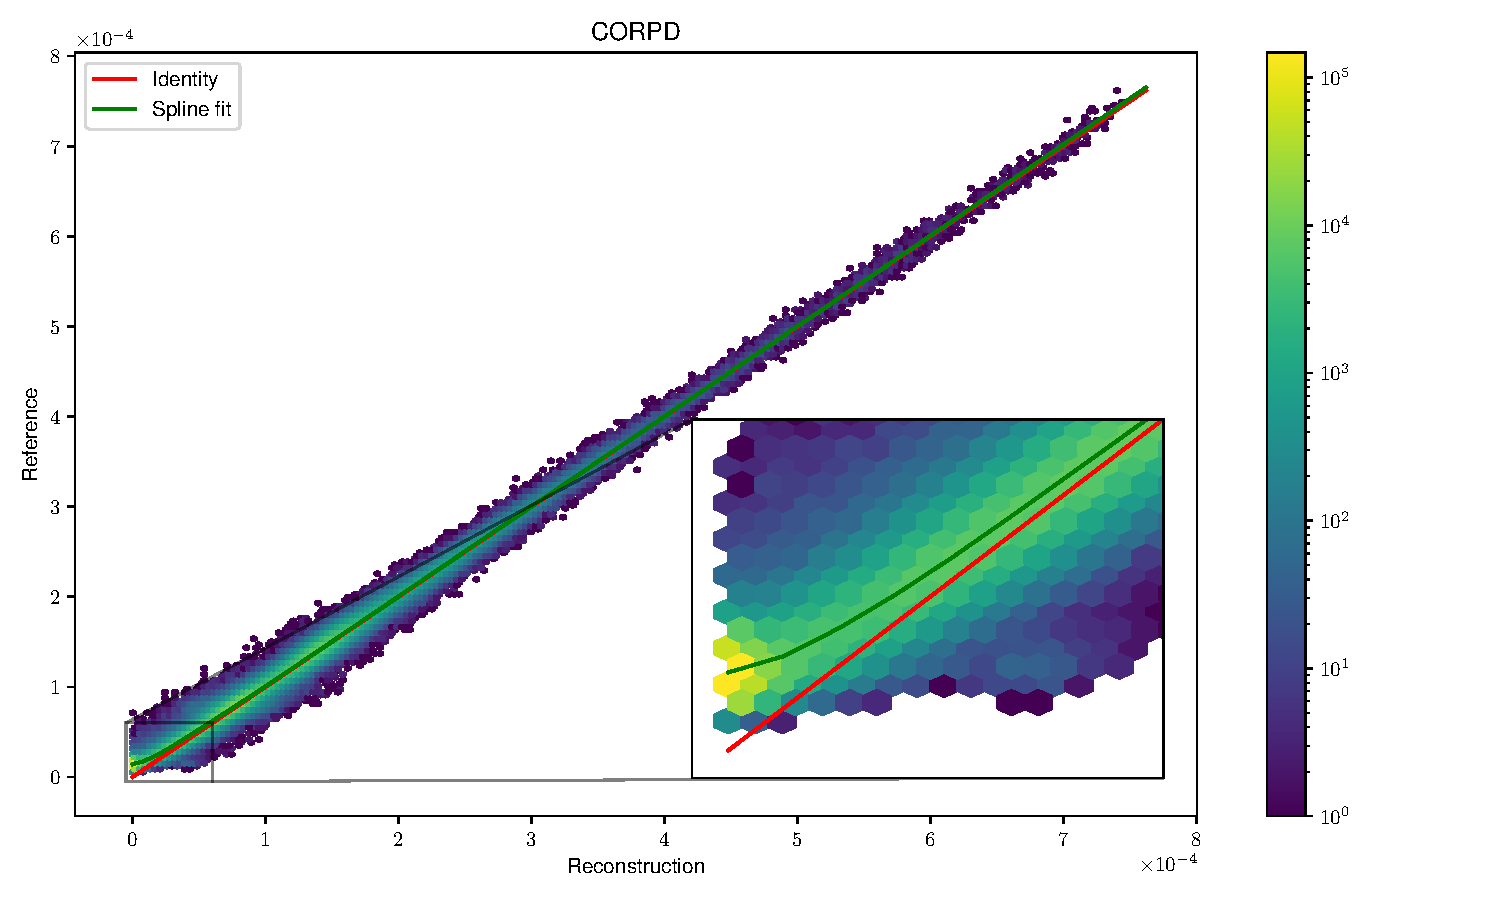
\includegraphics[width=.45\linewidth]{spline/spline}
	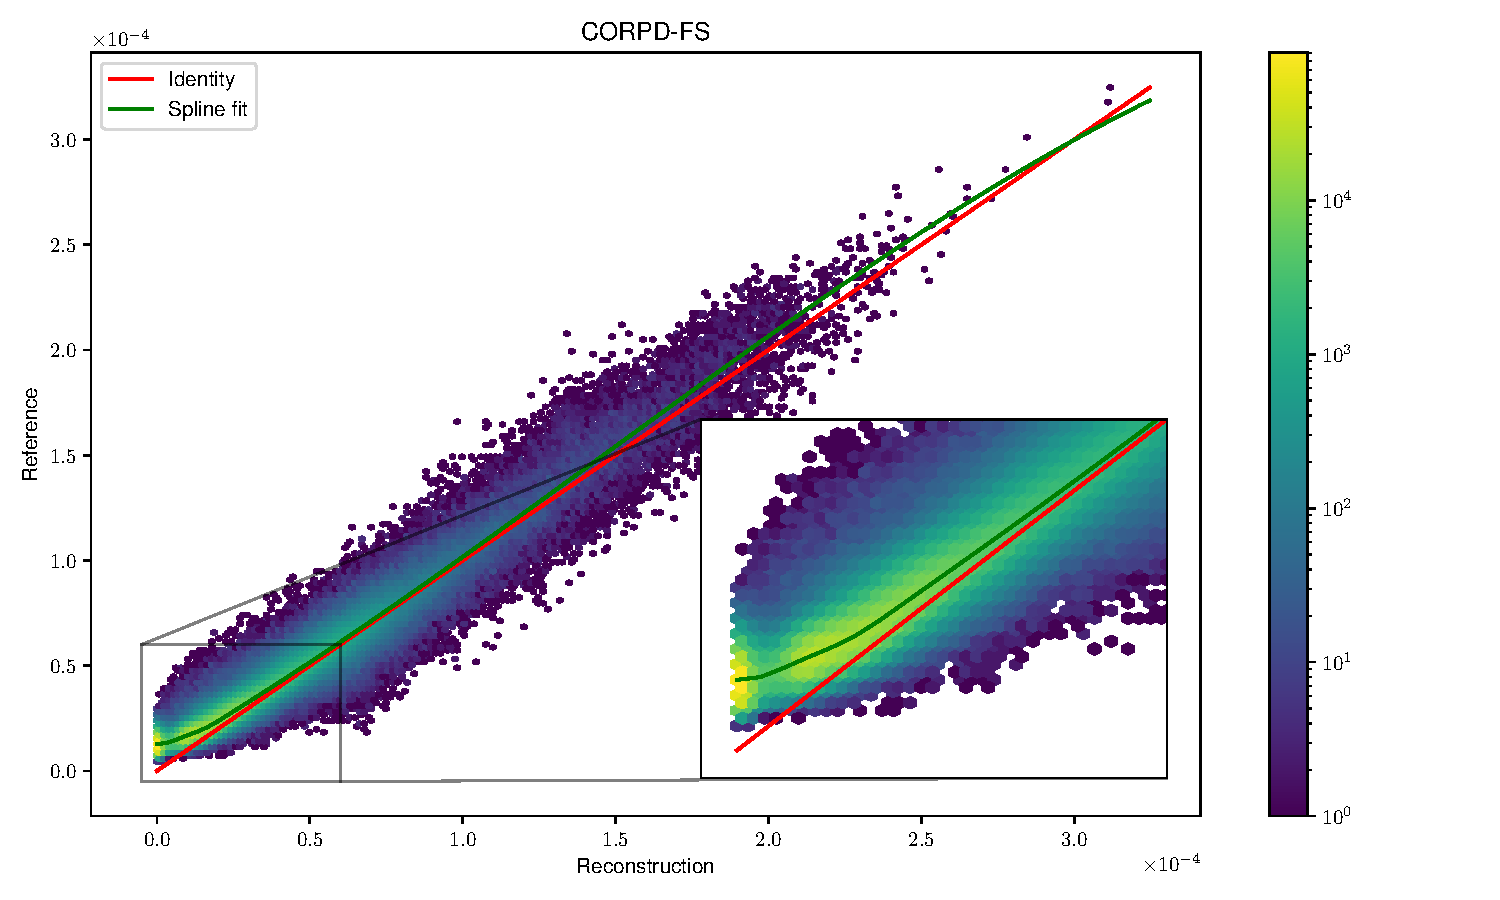
\includegraphics[width=.45\linewidth]{spline/spline-fs}
	\caption[Spline fit on the reconstructed versus the reference intensities]{%
		We account for for the systematic overestimation of the intensities near zero by utilizing a spline fit on the reconstructed intensities versus the reference intensities.
		The left plot shows the fit for the \gls{corpd} data, the right plot shows the fit for the \gls{corpdfs} data.
	}%
	\label{fig:splines}
\end{figure*}

To compute the \gls{mmse} estimate in the parallel imaging case, we fix the coil sensitivities to the \gls{map} estimate.
Thus, the iterations of the unadjusted Langevin algorithm take the form
\begin{equation}
	x^{k+\num{1}} = x^{k} + \tau \bigl( \sum_{i=\num{1}}^c \conj{\sigma_i} \odot (\Adjoint{\Fourier}\Adjoint{\Mask}(\Mask\Fourier(\sigma_i\odot x^k) - \Data_i)) + \lambda \Grad_{\num{1}} R(x^k, \theta) \bigr) + \sqrt{\num{2}\tau} z^k,
\end{equation}
where \( z^k \sim \NormalDistribution_{\num{0}, \Identity} \) and \( \sigma_{\num{1}}, \sigma_{\num{2}},\dotsc, \sigma_c \) are previously estimated coil sensitivities of the corresponding reconstruction problem.
The coil sensitivities may also be included in the Langevin procedure, but we empirically found no noticeable difference to fixing them.
We believe that this is due to the strong imposed spatial regularity, which corresponds to a \enquote{narrow} prior.

We evaluate the quality of the estimated coil sensitivities by computing the null-space residual~\cite{uecker_espirit_13}:
Let \( x_{\num{1}}, x_{\num{2}}, \dotsc, x_{c} \) the individual coil images from fully sampled data.
The null-space residual \( \rho_i \) of the \( i \)-th coil
\begin{equation}
	\rho_i = \frac{\sigma_i}{|\Sigma|^{\num{2}}_{\mathrm{rss}}} \sum_{j=\num{1}}^{c} \conj{\sigma}_j x_j - x_i,
	\label{eqq:null space residual}
\end{equation}
should only contain noise since \( x_i = \sigma_i x \) when \( \sigma_i \) is exact:
\begin{equation}
	\frac{\sigma_i}{|\Sigma|^{\num{2}}_{\mathrm{rss}}} \sum_{j=\num{1}}^{c} \conj{\sigma}_j x_j - x_i = 
	\frac{\sigma_i}{|\Sigma|^{\num{2}}_{\mathrm{rss}}} \sum_{j=\num{1}}^{c} \conj{\sigma}_j \sigma_j x - x_i = \sigma_i x - x_i = \num{0}.
\end{equation}
Thus, any residual signal in \( \rho_i \) points to sub-optimal sensitivity estimates.
In the results in~\cref{fig:nullspace}, for the sake of conciseness we do not inspect the null-space residual coil-wise, but instead show the \gls{rss} of the residual, \( \sqrt{\sum_{i=\num{1}}^c \abs{\rho_i}^{\num{2}}} \).
\subsection{Comparison and evaluation}
In the experiments on synthetic data, we compare against the fastMRI baseline method~\cite{zbontar_fastmri_2018} as well as the diffusion-based approach of~\cite{chung_scoremri_2022}.
To ensure a fair comparison, we trained the fastMRI baseline method on the subset of the fastMRI dataset detailed in~\cref{ssec:experimental data}.
To train the model, the data was constructed using a Cartesian frequency selection with acceleration \num{4} and \qty{8}{\percent} autocalibration lines;
other training hyperparameters are taken from the github repository of the authors.\footnote{Can be found at \url{https://github.com/facebookresearch/fastMRI}, accessed 2024--06--07.}
In contrast, training the diffusion model is extremely time- and resource intensive.
Thus, to avoid training a model we took the implementation as well as the weights of a trained model of the diffusion-based approach the github repository of the authors.\footnote{Can be found at \url{https://github.com/HJ-harry/score-MRI}, accessed 2024--06--07.}
We note that their model was trained on a larger corpus of data, as their training data includes the \gls{corpdfs} scans in addition to the \gls{corpd} scans.
As in their paper, we use \num{2000} steps in the reverse diffusion.
However, due to time and computational constraints, we limit our comparison to a subset of the validation data and hence provide results separately.

In the experiments on synthetic data as well as the parallel \gls{mri} experiments, we use the Charbonnier-smoothed isotropic total variation
\begin{equation}
	x \mapsto \lambda \sum_{i,j=\num{1}}^{m,n} \sqrt{\sum_{k=\num{1}}^{\num{2}} \bigl((\DiffOp x)_{i,j,k}\bigr)^{\num{2}} + \epsilon^{\num{2}}},
	\label{eq:charb}
\end{equation}
with \( \epsilon = \num{e-3} \) as a hand-crafted prior.
In the experiments on synthetic data, \( m = n = \num{320} \);
in the parallel \gls{mri} experiments, \( m = \num{640} \) and \( n = \num{368} \) or \( n = \num{372} \), depending on the width of the scan.
Thus, in contrast to our regularizer, we apply the Charbonnier-smoothed isotropic total variation regularizer to the entire image, not only to the central region.
We emphasize again that, for parallel \gls{mri}, we use the regularizer in conjunction with our proposed algorithm for join estimation of the image and the coil sensitivities.

As a state-of-the-art discriminative approach for parallel \gls{mri}, we compare against the end-to-end \gls{vn} approach from~\cite{sriram_endtoend_2020}.
The implementation was taken from the fastMRI github repository with default parameters.
As before, to ensure a fair comparison, the end-to-end \gls{vn} was trained on the subset of the fastMRI dataset detailed~\cref{ssec:experimental data}.
To train the model, the data was constructed using a Cartesian frequency selection with acceleration \num{4} and \qty{8}{\percent} autocalibration lines.

We compare the reconstructions quantitatively using the \gls{psnr}, \gls{nmse} and \gls{ssim}, see~\cref{def:psnr},~\cref{def:nmse}, and~\cref{def:ssim} respectively.
We compute the \gls{ssim} with the standard setup;
a \( \numproduct{7x7} \) uniform filter and parameters \( K_{\num{1}} = \num{0.01} \), \( K_{\num{2}} = \num{0.03} \).
We define the acceleration as the ratio of the image size and the acquired frequencies.
This is commonly done but only reflects the ill-posedness of the problem and not necessarily the achieved speed-up of a scan in practice.
The practical speed-up is determined by the alignment of the acquired frequencies with respect to each other due to the finite speed of the gradient coils in the \gls{mri} scanner.
The discussion of \gls{mri} physics and sequence design is out of the scope of this work, we refer to the thesis of Lazarus~\cite{lazarus_compressed_2018} for a discussion of sequence design in the context of accelerated \gls{mri}.
\section{Results}
\label{sec:results deep neural regularizer}
In this section, we first visualize preferred structures of our regularizer in~\cref{ssec:data independent analysis} using the unadjusted Langevin algorithm on the trained model.
Then, in~\cref{ssec:simulation study} we consider synthetic single-coil data, similar to~\cref{chap:regularizers}, leveraging the natural Bayesian interpretation to access posterior distributions for reconstructions.
This allows computation of different Bayesian estimators, such as \gls{map} and \gls{mmse} estimates, and visualization of pixel-wise marginal variance of the posterior distribution.
In~\cref{ssec:parallel imaging}, we apply our reconstruction algorithm and data-driven regularizer to parallel \gls{mri}, achieving state-of-the-art results with different frequency selections.
Here, our algorithm jointly estimates the image and coil sensitivities, showing superiority over offline estimation, especially with limited autocalibration data.
Finally, in~\cref{ssec:generalization}, we discuss generalization properties of the data-driven regularizer.
\subsection{Data-independent analysis}%
\label{ssec:data independent analysis}
In~\cref{chap:regularizers}, we reasoned about preferred structures of different ridge-type regularizers by visualizing filters and their corresponding potentials.
This is hardly possible with the deep neural regularizer, which includes \num{2368560} filters with nontrivial interaction\footnote{via cascaded nonlinearities and downsampling} and a final weighted sum containing \num{33600} weights.
However, we can visualize preferred structures by drawing samples from the Gibbs distribution (\cref{eq:gibbs}), making the model more interpretable compared to learned discriminative reconstruction approaches, thus facilitating clinical adoption.

Additionally, we can \emph{visualize the density} of the Gibbs distribution around the samples.
The local regularization landscape provides insights into properties such as (local) convexity, generalization capabilities, and adversarial robustness~\cite{Stutz_2021_adversarial}.
To visualize the (\numproduct{320x320})-dimensional landscape, we follow~\cite{li_2018_visualizing}:
Let \( x^{\num{0}}, x^{\num{1}},\dotsc, x^K \in \R^{\numproduct{320x320}} \) be iterates in the unadjusted Langevin algorithm\footnote{we set \( K = \num{10000} \)}~\cref{eq:ula regularizer}, with \( x^{\num{0}} \) drawn from uniformly from \( \interval{\num{0}}{\num{1}}^{\numproduct{320x320}} \).
Let \( v_{\num{1}}, v_{\num{2}} \) be the first two principal directions of the point cloud \( \Set{x^{\num{0}} - x^{K};x^{\num{1}} - x^{K};\dotsc;x^{K-\num{1}} - x^{K}} \) and denote \( \bar{x} = \frac{1}{K-1} \sum_{k=\num{1}}^{K-\num{1}} x^{k} \).

In~\cref{fig:mri sampling deep neural regularizers} we show\footnote{%
	\( T = \num{7} \) yields visually pleasing results.
	This scaling is arbitrary; it can make the density more or less peaky.
	In the context of a reconstruction problem, it is related to the regularization parameter.
} \( \R^{\num{2}} \ni (\xi_{\num{1}}, \xi_{\num{2}}) \mapsto \exp \bigl( -R(\bar{x} + \xi_{\num{1}} v_{\num{1}} + \xi_{\num{2}} v_{\num{2}}) / T \bigr) \) along with the Langevin trajectory.
The samples from the Gibbs distribution closely resemble those from the reference distribution\footnote{%
	Samples from the reference distribution are shown in e.g.~\cref{fig:parallel imaging id}.
}, suggesting that the model accurately represents high-level statistics of the reference data.
For example, the knee is centered and the femur and tibia are visible and anatomically plausibly separated, surrounded by muscle- and fat tissue with blood vessels, reflecting plausible anatomy.
This empirical evidence suggests that the data-driven regularizer is a good model of the negative log prior, which is highly desirable in reconstruction problems with signals drawn from the reference distribution.
For out-of-distribution signals, the regularizer might impart features of the reference distribution, discussed further in \cref{ssec:generalization}.

The two-dimensional landscape appears smooth on the considered domain and almost log-concave around modes of the Gibbs distribution, indicating that the high-dimensional landscape is also reasonably well-behaved.
This is corroborated by the ease of optimization: For all reconstruction tasks, we only need \num{50} to \num{100} iterations of \gls{ipalm}.
\begin{figure*}
	\centering
	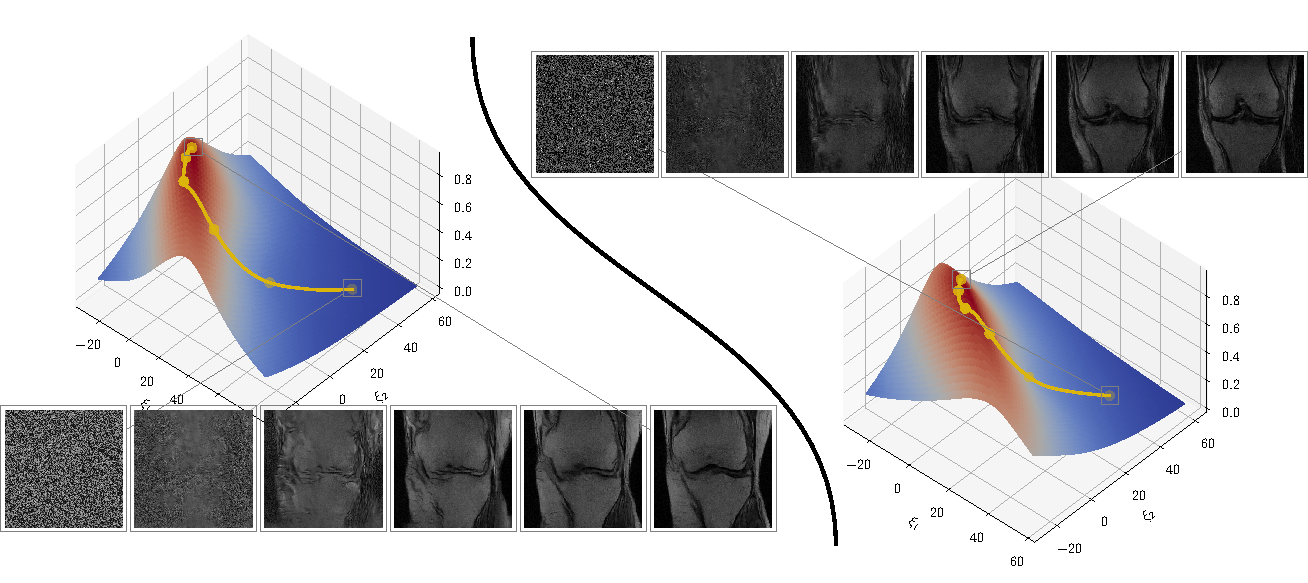
\includegraphics[width=\linewidth]{mri-sampling}
	\caption[Sampling a deep neural regularizer]{%
		We visualize preferred structures of the regularizer via \gls{mcmc} sampling.
		Uniform noise is unlikely under the deep neural regularizer---natural anatomical structures are very likely.
		The golden line is the trajectory of the unadjusted Langevin algorithm.
	}%
	\label{fig:mri sampling deep neural regularizers}
\end{figure*}
\subsection{Simulation study}%
\label{ssec:simulation study}
This chapter' contributions include designing and training the regularizer, and developing the algorithm for joint nonlinear inversion.
In this section, we focus on the data-driven regularizer by constructing a reconstruction problem that does not require coil sensitivity estimation.
Details of this construction and reference methods are provided in \cref{ssec:simulation study};
here, we state that we have access to data \( \Data \) given by
\begin{equation}
	\Data = \Mask \Fourier x + \Noise,
\end{equation}
where the aim is to recover the underlying signal \( x \in \R^{\numproduct{320x320}} \).
Crucially, the random variable of the underlying signal \( x \) is distributed as \( p_X \), the reference distribution on which the regularizer was trained.
We will demonstrate that for different frequency selection operators, encoded in \( \Mask \), the optimization problem
\begin{equation}
	\argmin_{x \in \R^{\numproduct{320x320}}} \Half \norm{\Mask\Fourier x - y}^{\num{2}} + \lambda R(x, \theta)
\end{equation}
yields satisfactory reconstructions.\footnote{%
	In this respect, there is also nothing special about the Fourier transform \( F \).
	Indeed, the regularizer will work well for any forward operator (Radon imaging, superresolution, etc.), so long as the underlying signal is drawn from the reference distribution.
}

We consider four different frequency selection operators:
\begin{enumerate}
	\item A random selection with acceleration \num{3},
	\item a Cartesian selection with a densely samples frequencies in the phase encoding direction, \qty{8}{\percent} autocalibration lines, and acceleration \num{4},
	\item a spiral selection with acceleration \num{5}, and
	\item a radial selection with acceleration \num{6}.
\end{enumerate}
These are visualized in in~\cref{fig:simulation study masks}.
\begin{figure*}
	\centering
	\begin{tikzpicture}
		\foreach [count=\isampling] \sampling/\anno in {random/Random (\num{3}), cartesian/Cartesian (\num{4}), spiral/Spiral (\num{5}), radial/Radial (\num{6})}
		{
			\node at (4.25*\isampling, 0) {\includegraphics[height=4cm]{single-coil-synthetic/\sampling/mask}};
			\node at (4.25*\isampling, 2.3) {\anno};
		}
	\end{tikzpicture}
	\caption[Frequency selection in the synthtetic experiments]{%
		A visualization of the frequency selection operators in the synthetic experiments:
		Low frequencies are understood to be in the center.
		Frequencies overlaid with a white pixel are understood to be present in the data, frequencies overlaid with a black pixel are not present in the data.
		With the random frequency selection, in contrast to all others, low frequencies are not more densely sampled.
		The number in parenthesis shows the acceleration, i.e.\ the number of all possible frequencies divided by the number of selected frequencies.
	}
	\label{fig:simulation study masks}
\end{figure*}

Qualitative reconstruction results for the different reconstruction problems are shown in~\cref{fig:simulation study}, corresponding quantitative results in terms of \gls{psnr}, \gls{nmse}, and \gls{ssim} in~\cref{tab:simulation results}.
The table also shows the number of learnable parameters and the reconstruction time.

We start with the prototypical reconstruction problem, Cartesian frequency selection with \qty{8}{\percent} autocalibration lines and acceleration \num{4}, shown in the second row.
This setup matches the training conditions of the discriminative UNet, resulting in satisfactory reconstructions.
However, even in this case the network hallucinates structures into the reconstruction that are not reflected in the data; an example is highlighted in~\cref{fig:simulation study}.\footnote{%
	Recall that data consistency is not explicitly enforced here.
	See also the previous discussion on the pitfalls of discriminative signal recovery in~\cref{sec:discriminative pitfalls}.
}
The isotropic \gls{tv} regularizer reconstruction shows typical back-folding artifacts, and increasing the regularization would lead to significant loss of detail.
Our data-driven regularizer produces reconstructions qualitatively (at least) on par with the discriminative U-Net.
Quantitatively, our reconstructions consistently beat the reference methods.
In particular, the our \gls{mmse} reconstruction beats the discriminative UNet by over \qty{2}{\decibel} in \gls{psnr}, even though the UNet was specifically trained for this task.
Generally, the \gls{mmse} estimate is superior to the \gls{map} estimate quantitatively and qualitatively, which is expected by the discussion on Bayes estimates in~\cref{chap:intro}.
\begin{figure*}
	\centering
	\tikzexternaldisable%
	\begin{tikzpicture}
		\def\cherries{{"file1002546.h5","file1001331.h5","file1001687.h5","file1002351.h5"}}
		\def\spyoff{{{-0.8cm,0.5cm},{0.75cm,0.3cm},{0.4cm,-0.3cm},{-.7cm,-1.0cm}}}
		\foreach [count=\isampling] \sampling/\sanno in {random/Random (3), cartesian/Cartesian (4), spiral/Spiral (5), radial/Radial (6)}
		{
			\pgfmathsetlengthmacro{\yy}{-\isampling * (\wwidth + \wwidth / 2 + \vpad)}
			\node [rotate=90,overlay] at (1.2, \yy) {\sanno};
			\pgfmathsetmacro{\spyxoff}{\spyoff[\isampling-1][0]}
			\pgfmathsetmacro{\spyyoff}{\spyoff[\isampling-1][1]}
			\pgfmathsetmacro{\cherry}{\cherries[\isampling-1]}
			\foreach [count=\imethod] \method/\manno in {%
				{zero_filled}/\glsxtrshort{zf},
				tv/\glsxtrshort{tv},
				unet/{U-Net},
				ours/{Ours (\glsxtrshort{map})},
				{mean}/{Ours (\glsxtrshort{mmse})},
				ground_truth/Reference%
			} {
				\pgfmathsetlengthmacro{\xx}{\imethod * (\wwidth + \hpad)}
				\ifthenelse{\isampling=1}{\node at (\xx, -\wwidth / 2 - 1cm) {\manno};}{}
				\ifthenelse{\imethod=5}{%
					\def\ourpath{single-coil-synthetic/posterior/\sampling/\cherry}
				}{%
					\def\ourpath{single-coil-synthetic/\sampling/\cherry}
				}
				\pgfmathsetlengthmacro{\xxspy}{\xx + \spyxoff}
				\pgfmathsetlengthmacro{\yyspy}{\yy + \spyyoff}
				\coordinate (onn) at (\xxspy, \yyspy);
				\ifthenelse{\imethod=6}{}{
				\begin{scope}[mrispy]
					\node [inner sep=0, outer sep=0] at (\xx, \yy) {\includegraphics[angle=180,origin=c,width=\wwidth]{\ourpath/d_\method}};
					\spy on (onn) in node at (\xx + \wwidth / 2 / 2, \yy - 1.5 * \wwidth / 2);
				\end{scope}}
				\begin{scope}[mrispy]
					\node[inner sep=0, outer sep=0] at (\xx, \yy) {\includegraphics[angle=180,origin=c,width=\wwidth]{\ourpath/\method}};
					\spy on (onn) in node at (\xx - \wwidth / 2 / 2, \yy - 1.5 * \wwidth / 2);
				\end{scope}
			}
		}
		\foreach \imethod in {1,...,6}{
			\pgfmathsetlengthmacro{\xx}{\imethod * (\wwidth + \hpad) - .8cm}
			\draw[ultra thick, -Stealth, white] (\xx, -7.7) -- ++(-.3, .4);
		}
		\foreach \imethod in {1,...,6}{
			\pgfmathsetlengthmacro{\xx}{\imethod * (\wwidth + \hpad) - .6cm}
			\draw[ultra thick, -Stealth, white] (\xx, -11.4) -- ++(.3, -.4);
		}
	\end{tikzpicture}
	\tikzexternalenable%
	\caption[Qualitative results for the synthetic experiments]{%
		Results on synthetic single-coil data.
		First row:
		Random frequency selection with acceleration \num{3}.
		Second row:
		Cartesian frequency selection acceleration \num{4} and \qty{8}{\percent} autocalibration lines.
		Third row:
		Spiral frequency selection with acceleration \num{5}.
		Fourth row:
		Radial frequency selection spokes with acceleration \num{6}.
		A visualization of the frequency selection operators can be seen in~\cref{fig:simulation study masks}.
		The inlays show a detailed zoom and the magnitude of the difference to the reference (\num{0}~\protect\drawcolorbar~\num{0.2}).
		The white arrow highlights features hallucinated by the discriminative UNet.
		This is especially notable in the second row (Cartesian frequency selection), where the reconstruction task corresponds to the training setup.
		Best viewed electronically.
	}%
	\label{fig:simulation study}
\end{figure*}
\begin{table*}
	\centering
	\caption[Quantitative results for synthetic experiments in MRI]{%
		Quantitative results for the synthetic experiments with different frequency selections.
		The rows alternate between \gls{psnr} (P, \( \uparrow\)), \gls{nmse} (N, \( \downarrow\)), and \gls{ssim} (S, \( \uparrow\)).
		Acc. is the acceleration, bold typeface indicates the best method.
		The comparison against the ScoreMRI method of~\cite{chung_scoremri_2022} is shown separately because the evaluation was done on only on a subset of the data.
	}%
	\label{tab:simulation results}
	\begin{tabular}{lrl*{8}{S[text-series-to-math,table-format=2.2,round-mode=places,round-precision=2]}}
		\toprule
		& {\multirow{2}{*}{Acc.}} & & {\multirow{2}{*}{\glsxtrshort{zf}}} & {\multirow{2}{*}{\glsxtrshort{tv}}} & {\multirow{2}{*}{U-Net}} & \multicolumn{2}{c}{Ours} & {\multirow{2}{*}{ScoreMRI}} & \multicolumn{2}{c}{Ours} \\
		\cmidrule(lr){7-8}\cmidrule(lr){10-11}
		& & & & & & {\glsxtrshort{map}} & {\glsxtrshort{mmse}} & & {\glsxtrshort{map}} & {\glsxtrshort{mmse}} \\
		\cmidrule(r){1-8}\cmidrule(r){9-11}
		\multirow{3}{*}{Random} %
		& \multirow{3}{*}{\num{3}} & {P} & 12.931758880615234 & 20.806852340698242 & 19.52480125427246 & 30.8723201751709 & \bfseries 32.44416046142578 & 33.31 & 31.78 & \bfseries 34.76 \\
		& & {N}& \fpeval{100 * 0.6423648595809937} & \fpeval{100 * 0.10220915079116821} & \fpeval{100 * 0.12830260396003723} & \fpeval{100 * 0.013434510678052902} & \bfseries \fpeval{100 * 0.010225472040474415} & {---} & {---} & {---} \\
		& &{S}& 0.4817352294921875 & 0.7321547269821167 & 0.5721480846405029 & 0.8576399087905884 & \bfseries 0.9027918577194214 & {---} & {---} & {---}\\
		\cmidrule(r){1-8}\cmidrule(r){9-11}
		\multirow{3}{*}{Cartesian} %
		& \multirow{3}{*}{\num{4}} && 24.160869598388672 & 31.469541549682617 & 34.161155700683594 & 35.53403091430664 & \bfseries 36.168399810791016 & 34.65 & 34.97 & \bfseries 35.55 \\
		&       && \fpeval{100 * 0.059642061591148376} & \fpeval{100 * 0.008760045282542706} & \fpeval{100 * 0.004405752755701542} & \fpeval{100 * 0.003225221298635006} & \bfseries \fpeval{100 * 0.002839048160240054} & {---} & {---} & {---}\\
		&  && 0.704010546207428 & 0.853325366973877 & 0.8865730166435242 & 0.8949872851371765 & \bfseries 0.9105123281478882  & {---} & {---} & {---}\\
		\cmidrule(r){1-8}\cmidrule(r){9-11}
		\multirow{3}{*}{Spiral} %
		& \multirow{3}{*}{\( \approx \num{5} \)} && 21.210956573486328 & 31.248300552368164 & 27.76167869567871 & 35.35053253173828 & \bfseries 36.209625244140625 & 35.66 & 36.07 & \bfseries 37.00 \\
		&      && \fpeval{100 * 0.1024087592959404} & \fpeval{100 * 0.009196978993713856} & \fpeval{100 * 0.019011199474334717} & \fpeval{100 * 0.0033660277258604765} & \bfseries \fpeval{100 * 0.0028191949240863323}  & {---} & {---} & {---}\\
		&   && 0.617068350315094 & 0.84514981508255 & 0.7843644618988037 & 0.8829594850540161 & \bfseries 0.9014105200767517 & {---} & {---} & {---} \\
		\cmidrule(r){1-8}\cmidrule(r){9-11}
		\multirow{3}{*}{Radial} %
		& \multirow{3}{*}{\( \approx \num{6} \)} && 27.015140533447266 & 32.86052322387695 & 31.76373863220215 & 35.04103088378906 & \bfseries 35.46697998046875 & 34.98 & 36.02 & \bfseries 36.56 \\
		&      && \fpeval{100 * 0.03293876722455025} & \fpeval{100 * 0.006426490843296051} & \fpeval{100 * 0.007553369738161564} & \fpeval{100 * 0.0036013659555464983} & \bfseries \fpeval{100 * 0.0033337108325213194}  & {---} & {---} & {---}\\
		&   && 0.4817352294921875 & 0.7103990912437439 & 0.6549839973449707 & 0.8577146530151367 & \bfseries 0.8871539831161499  & {---} & {---} & {---} \\
		\cmidrule(r){1-8}\cmidrule(r){9-11}
		\multicolumn{3}{l}{Learnable parameters} & {0} & {0} & {\num[round-mode=places,round-precision=1]{4.963e8}} & \multicolumn{2}{c}{\num{2.1e7}} & {\num[round-mode=places,round-precision=1]{6.8e7}} & \multicolumn{2}{c}{\num{2.1e7}} \\
		\cmidrule(r){1-8}\cmidrule(r){9-11}
		\multicolumn{2}{l}{Time in seconds} && {\num[round-mode=places,round-precision=0]{2.624988555908203e-4}} & {\num[round-mode=places,round-precision=2]{0.5890867710113525}} & {\num[round-mode=places,round-precision=2]{0.09634160995483398}} & {\num{3.13}} & {\num{333.3}} & {\num{251.6}} & {\num{3.13}} & {\num{333.3}} \\\bottomrule
	\end{tabular}
\end{table*}%

The third row shows the reconstructions spiral frequency selection, with acceleration \num{5}.
The spirals sample low frequencies more densely compared to high frequencies.
Despite less data availability compared to the Cartesian case, the reconstruction obtained by the \gls{tv} regularizer shows less back-folding artifacts, likely due to the availability of more high-frequency data, especially horizontal frequencies (see the visualization of the frequency selection operators in~\cref{fig:simulation study masks}).
However, some back-folding artifacts remain, especially in the background.
The U-Net struggles to discriminate between details in the anatomy and back-folding artifacts in the intermediary zero-filling reconstruction, leading to unnatural reconstructions and loss of detail.
As an example, a large dark spot in the femur in the zero-filling reconstruction is interpreted as an anatomical detail and persists in the final reconstruction.
In contrast, our approach is able to faithfully reconstruct the knee with no visible artifacts.
The reconstructions obtained with the radial frequency selection shown in the fourth row are similar;
the radial frequency selection also samples low frequencies more densely compared to high frequencies.

In contrast, random frequency selection does not sample low frequencies more densely, which manifests in the zero-filling reconstruction by large-scale intensity shifts.
None of the reference methods can correct this:
The \gls{tv} regularizer can not resolve nonlocal dependencies, and the UNet fails to distinguish between anatomical features and back-folding artifacts in the intermediary reconstruction.
Our approach can restore knee's general shape and retains details present in the data, alleviating the need for frequency selection operators to densely sample low frequencies.

During the writing of the paper and the thesis, the use of diffusion models in inverse problems gained popularity.
We compare our approach to Chung and Ye's diffusion-based method~\cite{chung_scoremri_2022}.
However, since this approach is very time consuming, we limit the evaluation to a subset of the data used for the other models.
Quantitative results in~\cref{tab:simulation results} are shown separately; qualitative results in~\cref{fig:diffusion comparison}.
Our \gls{mmse} estimate consistently outperforms the diffusion-based approach, and our \gls{map} estimate is only inferior for the random frequency selection.
Computing the \gls{mmse} estimate takes only about \qty{30}{\percent} more time than computing one sample with the diffusion-based approach,\footnote{%
	This is in our particular setup, see the details in~\cref{ssec:details simulation study}.
}
while computing our \gls{map} estimate is about \num{80} times faster.
\begin{figure}
	\centering
	\def\spyoff{{%
		{-0.6,-0.1},%
		{0.65,0.3},%
		{-0.4,0.3},%
		{.7,.7}}%
	}
	\tikzexternaldisable
	\begin{tikzpicture}
		\foreach [count=\isampling] \sampling/\sanno in {random/Random (3), cartesian/Cartesian (4), spiral/Spiral (5), radial/Radial (6)}
		{
			\pgfmathsetlengthmacro{\yy}{-\isampling * (\wwidth + \wwidth / 2 + \vpad)}
			\node [overlay, rotate=90] at (1.2, \yy) {\sanno};
			\pgfmathsetmacro{\spyxoff}{\spyoff[\isampling-1][0]}
			\pgfmathsetmacro{\spyyoff}{\spyoff[\isampling-1][1]}
			\foreach [count=\imethod] \method/\manno in {%
				recon/{ScoreMRI},
				ours/Ours (\glsxtrshort{map}),
				mean/Ours (\glsxtrshort{mmse}),
				ground_truth/Reference%
			}{
				\pgfmathsetlengthmacro{\xx}{\imethod * (\wwidth + \hpad)}
				\ifthenelse{\isampling=1}{\node at (\xx, -\wwidth / 2 - 1cm) {\manno};}{}
				\coordinate (onn) at (\xx + \spyxoff, \yy + \spyyoff);
				\ifthenelse{\imethod=4}{}{
				\begin{scope}[mrispy]
					\node [inner sep=0, outer sep=0] at (\xx, \yy) {\includegraphics[angle=180,origin=c,width=\wwidth]{diffusion-comparison/\sampling/d_\method}};
					\spy on (onn) in node at (\xx + \wwidth / 2 / 2, \yy - 1.5 * \wwidth / 2);
				\end{scope}}
				\begin{scope}[mrispy]
					\node [inner sep=0, outer sep=0] at (\xx, \yy) {\includegraphics[angle=180,origin=c,width=\wwidth]{diffusion-comparison/\sampling/\method}};
					\spy on (onn) in node at (\xx - \wwidth / 2 / 2, \yy - 1.5 * \wwidth / 2);
				\end{scope}
			}
		}
	\end{tikzpicture}
	\tikzexternalenable
	\caption[Qualitative compoarison against diffusion models]{%
		Qualitative comparison against~\cite{chung_scoremri_2022} on in-distribution data:
		First row:
		Random frequency selection with acceleration \num{3},
		Second row:
		Cartesian frequency selection with \qty{8}{\percent} autocalibration lines and acceleration \num{4},
		Third row:
		Spiral frequency selection with acceleration \num{5},
		Fourth row:
		Radial frequency selection with acceleration \num{6}.
		The inlays show a detail zoom, and the magnitude of the difference to the reference (\num{0}~\protect\drawcolorbar~\num{0.2}).
	}%
	\label{fig:diffusion comparison}
\end{figure}

Our approach allows us to trade off reconstruction quality with computational time:
The \gls{mmse} estimate gracefully approaches the \gls{map} estimate as we take fewer and fewer samples, since we initialize the unadjusted Langevin algorithm with the \gls{map} estimate.
Although significant advances have been made to speed up diffusion models (see e.g.~\cite{Karras2022edm,chung2022come}), they are in general still slower.
\subsection{Uncertainty quantification}
The strict Bayesian approach taken in this thesis allows access to a \emph{posterior distribution} of reconstructions for a datum.
In the previous section, we computed the \gls{map} as well as the \gls{mmse} estimate of this distribution.
The \gls{mmse} estimate is the expectation (\cref{def:expectation}, the first moment) of the posterior.
In this section, we discuss higher order moments, such as the variance~\cref{def:variance}---the second moment.

Computing the second moment of the posterior distribution for our reconstruction problems is infeasible:
This moment is described by \( (\numproduct{320x320})\times(\numproduct{320x320}) = \num{10485760000} \) real numbers.
Therefore, we restrict our focus to the pixel-wise marginal variance, as is commonly done in this context~\cite{chung_scoremri_2022,Narnhofer2024,Pereyra2023}.
Notably, computing the pixel-wise marginal variance does not incur additional computational cost when computing the \gls{mmse} estimate:
The \gls{mmse} estimate is obtained by taking the pixel-wise average of all samples from the posterior, while the pixel-wise marginal variance is computed by taking the pixel-wise variance.

In~\cref{fig:simulation study posterior sampling}, we present the \gls{mmse} estimate along with the pixel-wise marginal variance and the magnitude of the error for the same reconstruction problems discussed in the previous section.
As expected, the pixel-wise marginal variance increases with the acceleration:
random frequency selection with acceleration \num{3} shows the smallest variance, while radial frequency selection with acceleration \num{6} shows the highest.
The additional variance information can aid clinicians in decision making and enhance interpretability of the results.
In addition, it can be combined with conformal prediction techniques to provide coverage guarantees for error bounds, as proposed by Narnhofer, Habring, Holler, and Pock~\cite{Narnhofer2024}.
\begin{figure*}
	\tikzexternaldisable%
	\begin{tikzpicture}
	\def\cherry{file1002382.h5}
	\def\spyxoff{-.8cm}
	\def\spyyoff{-.3cm}
	\foreach [count=\icc] \cherry/\xshift in {file1000702.h5/0, file1000831.h5/8.5cm}{
		\begin{scope}[xshift=\xshift]
			\foreach [count=\isampling] \sampling/\sanno in {random/Random (3), cartesian/Cartesian (4), spiral/Spiral (5), radial/Radial (6)}
			{
				\pgfmathsetlengthmacro{\yy}{-\isampling * (\wwidth + \wwidth / 2 + \vpad)}
				\ifthenelse{\icc=1}{\node [rotate=90, overlay] at (1.2, \yy) {\sanno};}{}
					\foreach [count=\iimname] \imname/\manno in {mean/{\(\Expectation[X\mid z]\)}, var/{\( (\Variance[X\mid z])_{i, j} \)}, error_scaled/Error} {
					\pgfmathsetlengthmacro{\xx}{\iimname * (\wwidth + \hpad - 1mm)}
					\ifthenelse{\isampling=1}{\node at (\xx, -\wwidth / 2 - 1cm) {\manno};}{}
					\coordinate (onn) at (\xx + \spyxoff, \yy + \spyyoff);
					\begin{scope}[spy using outlines={width=\wwidth, height=\spysize, rectangle, maincolor, magnification=3}]
						\node [inner sep=0, outer sep=0] at (\xx, \yy) {\includegraphics[angle=180,origin=c,width=\wwidth]{posterior/\sampling/\cherry/\imname}};
						\spy on (onn) in node at (\xx, \yy - 1.5 * \wwidth / 2);
					\end{scope}
				}
			}
		\end{scope}
	}
	\end{tikzpicture}%
	\tikzexternalenable%
	\caption[Pixel-wise marginal variance]{%
		The \gls{mmse} estimate along with the pixel-wise marginal variance (\( \num{0}~\protect\drawcolorbar~\num{0.0025} \)) and the magnitude of the error to the reference signal.
		First row:
		Random frequency selection with acceleration \num{3}.
		Second row:
		Cartesian frequency selection with \qty{8}{\percent} autocalibration lines and acceleration \num{4}.
		Third row:
		Spiral frequency selection with acceleration \num{5}.
		Fourth row:
		Radial frequency selection with acceleration \num{6}.
		The variance increases as less data is available and could be used to obtain coverage guarantees for error bounds~\cite{Narnhofer2024}.
		A visualization of the frequency selection operators can be seen in~\cref{fig:simulation study masks}.
	}%
	\label{fig:simulation study posterior sampling}
\end{figure*}%

In our proof-of-concept paper dealing with Radon imaging, we investigated the possibility of using the pixel-wise marginal variance for pathology detection.
We briefly discuss the results here, referring to the publication~\cite{zach_computed_2021} for more details on the experimental setup and discussion of the results.
We introduce an artificial structure (a \enquote{pathology}) in the image by overlaying the \enquote{cameraman} onto the anatomy.
Comparing the pixel-wise marginal variance in~\cref{fig:ct pathology}, the variance around the artificial structures is significantly higher than in the reference scan.
This suggests the potential for developing a pathology detection system based on this variance.
Pathologies, seen as anomalies, align with the broader field of anomaly detection methods discussed in~\cite{10.1145/3439950}.
\begin{sidefigure}
	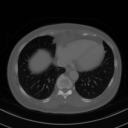
\includegraphics[width=\marginparwidth]{ct/clean/scan}
	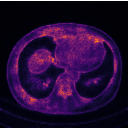
\includegraphics[width=\marginparwidth]{ct/clean/std}
	\rule[2mm]{\marginparwidth}{.3em}\\
	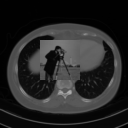
\includegraphics[width=\marginparwidth]{ct/cameraman/scan}
	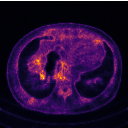
\includegraphics[width=\marginparwidth]{ct/cameraman/std}
	\caption[Pathology detection via posterior variance]{The pixel-wise marginal variance in the region around the unnatural cameraman is significantly higher than in the reference scan.}%
	\label{fig:ct pathology}
\end{sidefigure}
\subsection{Parallel imaging}%
\label{ssec:parallel imaging}
The previous sections outlined the benefits of our data-driven regularizer.
In this section, we demonstrate that our proposed algorithm, combined with the data-driven regularizer, achieves state-of-the-art results in parallel \gls{mri} reconstruction problems encountered in clinical practice.
We first focus on the reconstructions, showing excellent results for numerous frequency selection operators.
Then, we examine the coil sensitivity estimates, highlighting the advantages of our approach over offline coil sensitivity estimation, especially when little data are available.

We assume that the data \( z_{\num{1}}, z_{\num{2}}, \dotsc, z_c \) of \( c \in \mathbb{N} \) coils are given by~\cref{eq:data for parallel imaging}, with both the coil sensitivities and the underlying signal are unknown.
As in previous sections, we assume that the underlying signal comes from the same distribution that the regularizer was trained on, \( \DensityFunctionX \).
We consider five different frequency selection operators:
\begin{enumerate}
	\item A Cartesian selection with densely sampled frequencies in the phase-encoding direction, \qty{8}{\percent} autocalibration lines, and acceleration \num{4},\label{item:cartesian frequencies}
	\item the same setup as in~\cref{item:cartesian frequencies} but with swapped phase-encoding direction,
	\item the same setup as in~\cref{item:cartesian frequencies} but with \qty{4}{\percent} autocalibration lines,
	\item a two-dimensional Gaussian selection with acceleration \num{8}, and
	\item a radial selection with acceleration \num{11}.
\end{enumerate}
The two-dimensional Gaussian selection is understood as assigning each frequency a probability of being included that falls off as a Gaussian from the center.
These are visualized in~\cref{fig:parallel imaging masks}.
\begin{figure*}
	\centering
	\begin{tikzpicture}
		\foreach [count=\isampling] \sampling/\sanno in {%
			cartesian/{Cartesian (\num{4})},
			{cartesian_rot90}/{Cartesian\textsuperscript{\qty{90}{\degree}} (\num{4})},
			{cartesian_4}/{Cartesian\textsuperscript{\qty{4}{\percent}} (\num{4})},
			gaussian2d/{Gaussian (\num{8})},%
			radial/{Radial (\num{11})}%
		}{%
			\node at (\isampling*3.25, 0) {\includegraphics[height=5cm]{validation/\sampling/mask}};
			\node at (3.25*\isampling, 2.8) {\sanno};
		}
	\end{tikzpicture}
	\caption[Frequency selection in parallel imaging]{%
		A visualization of the frequency selection operators we consider in the parallel imaging experiments:
		Low frequencies are understood to be in the center.
		Frequencies overlaid with a white pixel are understood to be present in the data, frequencies overlaid with a black pixel are not present in the data.
		The number in parenthesis shows the acceleration, i.e.\ the number of all possible frequencies divided by the number of selected frequencies.
	}%
	\label{fig:parallel imaging masks}
\end{figure*}

We present qualitative reconstruction results for the different reconstruction problems in~\cref{fig:parallel imaging id}, and the corresponding quantitative results in terms of \gls{psnr}, \gls{nmse}, and \gls{ssim} in~\cref{tab:parallel imaging}.

The first row of~\cref{fig:parallel imaging id} shows the prototypical Cartesian frequency selection with \qty{8}{\percent} autocalibration lines and acceleration \num{4}, corresponding to the training setup of the discriminative end-to-end \gls{vn} of~\cite{sriram_endtoend_2020}.
Consequently, the reconstructions are satisfactory, with the \gls{vn} achieving the best quantitative results with a \gls{psnr} of \qty{36.92}{\decibel} on the test set.
Our method also achieves competitive results with a \gls{psnr} of \qty[round-mode=places,round-precision=2]{35.22513961791992}{\decibel}.
This is expected, as generative approaches typically do not outperform discriminative counterparts.

The benefits of our approach become apparent when we slightly change the frequency selection:
the performance of the end-to-end \gls{vn} deteriorates significantly when the phase-encoding direction is swapped, or when less autocalibration lines are acquired.
Notably, the acceleration remains \emph{fixed}.
These minimal changes in the frequency selection cause the end-to-end \gls{vn} to struggle with back-folding artifacts or introduces severe hallucinations.
In contrast, our approach maintains stable performance across all tasks, reflected in the quantitative evaluation in \cref{tab:parallel imaging}.
For example, the \gls{psnr} of the reconstructions of the end-to-end \gls{vn} drops by \qty{12.20}{\decibel} when phase-encoding direction is swapped, whereas our approach's \gls{psnr} increases by \qty{1}{\decibel}.\footnote{%
	Due to the knee's longitudinal arrangement in the scanner, swapped phase encoding is advantageous because more horizontal high-frequency information is available, see the visualization in~\cref{fig:parallel imaging masks}.
}
When reducing autocalibration lines from \qty{8}{\percent} to \qty{4}{\percent}, the \gls{psnr} of the end-to-end \gls{vn} drops by \qty{4.76}{\decibel}, whereas the \gls{psnr} of our approach remains almost constant.\footnote{It increases by \qty{0.1}{\decibel}.}

\begin{figure*}
	\centering
	\tikzexternaldisable%
	\begin{tikzpicture}
		\def\cherries{{"file1001057.h5","file1002021.h5","file1001598.h5","file1002257.h5","file1001983.h5"}}
		\def\spyoff{{{0.65cm,0.3cm},{0.6cm,-0.7cm},{0.5cm,0.1cm},{.9cm,0.6cm},{0.2cm,0.9cm}}}
		\foreach [count=\isampling] \sampling/\sanno in {
			cartesian/Cartesian (\num{4}),
			{cartesian_rot90}/{Cartesian\textsuperscript{\qty{90}{\degree}} (\num{4})},
			{cartesian_4}/{Cartesian\textsuperscript{\qty{4}{\percent}} (\num{4})},
			gaussian2d/Gaussian (\num{8}),%
			radial/Radial (\num{11})%
		}{
			\pgfmathsetlengthmacro{\yy}{-\isampling * (\wwidth + \wwidth / 2 + \vpad)}
			\pgfmathsetmacro{\spyxoff}{\spyoff[\isampling-1][0]}
			\pgfmathsetmacro{\spyyoff}{\spyoff[\isampling-1][1]}
			\pgfmathsetmacro{\cherry}{\cherries[\isampling-1]}
			\foreach [count=\imethod] \method/\manno in {%
				{zero_filled}/\glsxtrshort{zf},
				tv/{\glsxtrshort{tv}},
				vn/{\glsxtrshort{vn}},
				ours/{Ours (\glsxtrshort{map})},
				ours_mmse/{Ours (\glsxtrshort{mmse})},
				ground_truth/Reference%
			}{
				\pgfmathsetlengthmacro{\xx}{\imethod * (\wwidth + \hpad)}
				\ifthenelse{\isampling=1}{\node at (\xx, -\wwidth / 2 - 1cm) {\manno};}{}
				\pgfmathsetlengthmacro{\xxspy}{\xx + \spyxoff}
				\pgfmathsetlengthmacro{\yyspy}{\yy + \spyyoff}
				\coordinate (onn) at (\xxspy, \yyspy);
				\ifthenelse{\imethod=6}{}{
				\begin{scope}[mrispy]
					\node [inner sep=0, outer sep=0] at (\xx, \yy) {\includegraphics[angle=180,origin=c,width=\wwidth]{validation/\sampling/\cherry/d_\method}};
					\spy on (onn) in node at (\xx + \wwidth / 2 / 2, \yy - 1.5 * \wwidth / 2);
				\end{scope}}
				\begin{scope}[mrispy]
					\node [inner sep=0, outer sep=0] at (\xx, \yy) {\includegraphics[angle=180,origin=c,width=\wwidth]{validation/\sampling/\cherry/\method}};
					\spy on (onn) in node at (\xx - \wwidth / 2 / 2, \yy - 1.5 * \wwidth / 2);
				\end{scope}
			}
			\ifthenelse{\boolean{bPrintVersion}}{%
				\node [rotate=-90, overlay] at (19.0, \yy) {\sanno};
			}{%
				\node [rotate=90, overlay] at (1.2, \yy) {\sanno};
			}
		}
	\end{tikzpicture}
	\tikzexternalenable%
	\caption[Qualitative results for parallel imaging on in-distribution data]{%
		Parallel imaging on in-distribution data:
		First row:
		\num{4}-fold Cartesian frequency selection with \qty{8}{\percent} autocalibration lines and acceleration \num{4}.
		Second row:
		As in the first row but with swapped phase encoding direction.
		Third row:
		As in the first row but with \qty{4}{\percent} autocalibration lines.
		Fourth row:
		2D Gaussian frequency selection with acceleration \num{8}.
		Fifth row:
		Radial frequency selection with acceleration \num{11}.
		The inlays show a detail zoom and the magnitude of the difference to the reference (\num{0}~\protect\drawcolorbar~\num{0.2}).
	}%
	\label{fig:parallel imaging id}
\end{figure*}
\begin{table*}
	\centering
	\caption[Quantitative results for parallel MRI on in- and out-of-distribution data]{%
		Quantitative results for parallel imaging with different frequency selections on in- and out-of-distribution data.
        The rows alternate between \gls{psnr}, \gls{nmse}, and \gls{ssim}.
		The \( \dagger \) column shows results using the \gls{corpd} \( \lambda \)-fit, while the \( * \) column has \gls{corpdfs}-adapted parameters (see~\cref{ssec:methods pi}).
	}%
	\label{tab:parallel imaging}
	\begin{tabular}{lrc*{10}{S[table-format=2.2,round-mode=places,round-precision=2]}}
        \toprule
		& & & \multicolumn{5}{c}{In-distribution (\glsxtrshort{corpd})} & \multicolumn{5}{c}{Out-of-distribution (\glsxtrshort{corpdfs})} \\
        \cmidrule(lr){4-8}\cmidrule(lr){9-13}
		& {\multirow{2}{*}{A}} & {\multirow{2}{*}{\glsxtrshort{acl}}} & {\multirow{2}{*}{\glsxtrshort{zf}}} & {\multirow{2}{*}{\glsxtrshort{tv}}} & {\multirow{2}{*}{\glsxtrshort{vn}}} & \multicolumn{2}{c}{Ours}  & {\multirow{2}{*}{\glsxtrshort{zf}}} & {\multirow{2}{*}{\glsxtrshort{tv}}} & {\multirow{2}{*}{\glsxtrshort{vn}}} & \multicolumn{2}{c}{Ours}\\
        \cmidrule(lr){7-8}\cmidrule(lr){12-13}
		& & & & & & \glsxtrshort{map} & \glsxtrshort{mmse} & &  & & {\( \dagger \)} & {\( * \)} \\
		\midrule
		\multirow{9}{*}{C} & \multirow{9}{*}{\num{4}} & \multirow{3}{*}{\qty{8}{\percent}} & 27.18990707397461 & 31.867795944213867 & \bfseries 36.92045211791992 & 35.22513961791992 & 35.27544403076172 & 26.091176986694336 & 31.302940368652344 & 29.998945236206055 & 30.602453231811523 & \bfseries 31.712961196899414 \\
		& & & \fpeval{100 * 0.0223829485476017} & \fpeval{100 * 0.007890134118497372} & \bfseries \fpeval{100 * 0.002435196889564395} & \fpeval{100 * 0.0036337128840386868} & \fpeval{100 * 0.003618051065132022} & \fpeval{100 * 0.05352313444018364} & \fpeval{100 * 0.01478771585971117} & \fpeval{100 * 0.023820199072360992} & \fpeval{100 * 0.019470086321234703} & \bfseries \fpeval{100 * 0.013532079756259918} \\
		& & & 0.7375055551528931 & 0.8079418540000916 & \bfseries 0.9163976311683655 & 0.88604736328125 & 0.8878628015518188 & 0.6760171055793762 & 0.7300366759300232 & \bfseries 0.7710118293762207 & 0.731391966342926 & 0.7327521443367004 \\
		\cmidrule{3-13}
		& & \multirow{3}{*}{\qty{8}{\percent}} %
	    & 31.12578582763672 & 33.03041076660156 & 24.720752716064453 & \bfseries 36.230690002441406 & 36.01150894165039 & 26.57789421081543 & 31.557456970214844 & 28.57035255432129 & 30.890687942504883 & \bfseries 31.652633666992188 \\
		& & & \fpeval{100 * 0.00931438896805048} & \fpeval{100 * 0.005917737260460854} & \fpeval{100 * 0.04011896252632141} & \bfseries \fpeval{100 * 0.0028249204624444246} & \fpeval{100 * 0.0029919317457824945} & \fpeval{100 * 0.051486801356077194} & \fpeval{100 * 0.014020383358001709} & \fpeval{100 * 0.028979137539863586} & \fpeval{100 * 0.022375022992491722} & \bfseries \fpeval{100 * 0.013702597469091415} \\
		& & & 0.8110671043395996 & 0.8260417580604553 & 0.670006275177002 & \bfseries 0.898271918296814 & \bfseries 0.8988670110702515 & 0.7056003212928772 & 0.7315869927406311 & 0.707637369632721 & \bfseries 0.7516953945159912 & 0.7289502024650574\\
		\cmidrule{3-13}
		 & & \multirow{3}{*}{\qty{4}{\percent}} %
		& 24.141496658325195 & 25.81011390686035 & 32.16292190551758 & \bfseries 35.33468246459961 & 35.224971771240234 & 24.9786319732666 & 29.91111183166504 & 29.117982864379883 & 29.933029174804688 & \bfseries 31.255582809448242 \\
		& & & \fpeval{100 * 0.04508989304304123} & \fpeval{100 * 0.034832630306482315} & \fpeval{100 * 0.0069937678053975105} & \bfseries \fpeval{100 * 0.0035170933697372675} & \fpeval{100 * 0.0036184450145810843} & \fpeval{100 * 0.06647732108831406} & \fpeval{100 * 0.020912175998091698} & \fpeval{100 * 0.027873607352375984} & \fpeval{100 * 0.029169296845793724} & \bfseries \fpeval{100 * 0.015278858132660389}\\
		& & & 0.6923396587371826 & 0.6951988935470581 & \bfseries 0.8927095532417297 & \bfseries 0.8880932331085205 & \bfseries 0.8893769383430481 & 0.6545588970184326 & 0.7075069546699524 & \bfseries 0.7572644352912903 &  0.7270150184631348 & 0.7248818874359131\\
		\midrule
		\multirow{3}{*}{R} & \multirow{3}{*}{\num{11}} & \multirow{3}{*}{---} %
		& 28.76137351989746 & 32.46963882446289 & 20.558855056762695 & \bfseries 34.45677947998047 & 34.1624641418457 & 25.058237075805664 & 31.15333366394043 & 26.257211685180664 & \bfseries 31.433210372924805 & 31.355825424194336\\
		& & & \fpeval{100 * 0.015698831528425217} & \fpeval{100 * 0.006666331551969051} & \fpeval{100 * 0.10128451883792877} & \bfseries \fpeval{100 * 0.004226132296025753} & \fpeval{100 * 0.0045379577204585075} & \fpeval{100 * 0.07370038330554962} & \fpeval{100 * 0.015259397216141224} & \fpeval{100 * 0.049717504531145096} & \bfseries \fpeval{100 * 0.014507188461720943} & \fpeval{100 * 0.01571197621524334}\\
		& & & 0.7465711236000061 & 0.8061649203300476 & 0.6916904449462891 & \bfseries 0.8565337657928467 & \bfseries 0.8555713295936584 & 0.6186882853507996 & 0.712673008441925 & 0.6861987709999084 & \bfseries 0.7252629399299622 & 0.7009592056274414\\
		\midrule
		\multirow{3}{*}{G} & \multirow{3}{*}{8} & \multirow{3}{*}{---} & 32.0957145690918 & 34.1363525390625 & 20.741687774658203 & 35.34770965576172 & \bfseries 35.412174224853516 & 26.754220962524414 & 31.52347755432129 & 23.461977005004883 & 31.874441146850586 & \bfseries 32.09153366088867\\
		& & & \fpeval{100 * 0.007424597162753344} & \fpeval{100 * 0.004535387735813856} & \fpeval{100 * 0.09953409433364868} & \bfseries \fpeval{100 * 0.003436274826526642} & \bfseries \fpeval{100 * 0.003413973143324256} & \fpeval{100 * 0.05457334592938423} & \fpeval{100 * 0.014161386527121067} & \fpeval{100 * 0.09929478168487549} & \fpeval{100 * 0.01432089228183031} & \bfseries \fpeval{100 * 0.0124507499858737}\\
		& & & 0.8387000560760498 & 0.8521340489387512 & 0.6813638210296631 & 0.8809531927108765 & \bfseries 0.8852419853210449 & 0.7052920460700989 & 0.7458847165107727 & 0.6833181977272034 & \bfseries 0.7555358409881592 & 0.7461521029472351\\
		\bottomrule
	\end{tabular}
\end{table*}

The situation is similar for the two-dimensional Gaussian and radial frequency selection, but the artifacts introduced by the end-to-end \gls{vn} become even more pronounced.
This is due the sensitivity estimation sub-network in the end-to-end \gls{vn} failing, which assumes a densely samples low frequencies, similarly to offline coil sensitivity estimation algorithms.
In addition, the image estimation sub-network is confronted with unseen features since it is coupled to the sensitivity estimation network.
Quantitatively, the end-to-end \gls{vn} performs much worse than the \gls{tv} reconstruction for these frequency selections, although the \gls{tv} reconstructions appear overly smooth.
Our approach satisfactorily reconstructs the image, yielding the best performance both quantitatively and qualitatively.

In the third row of~\cref{fig:parallel imaging id}, we highlight a failure case of our algorithm:
In the second columns, with the Charbonnier-smoothed isotropic \gls{tv} regularizer, parts of the details of the anatomy have \enquote{slipped} into the coil sensitivities, some of which we show in~\cref{fig:failure case coil sensitivities}.
\begin{sidefigure}
	\centering
	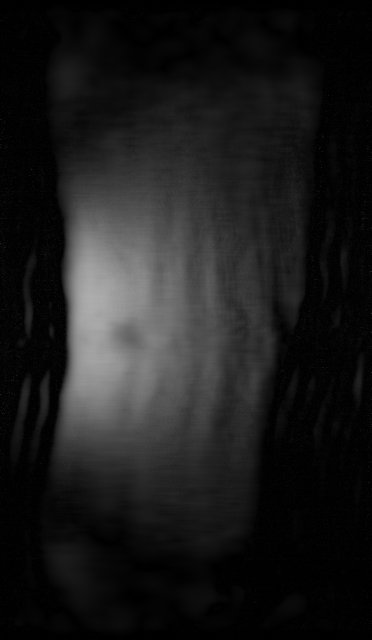
\includegraphics[width=.45\marginparwidth]{failure/coil_ims_05}
	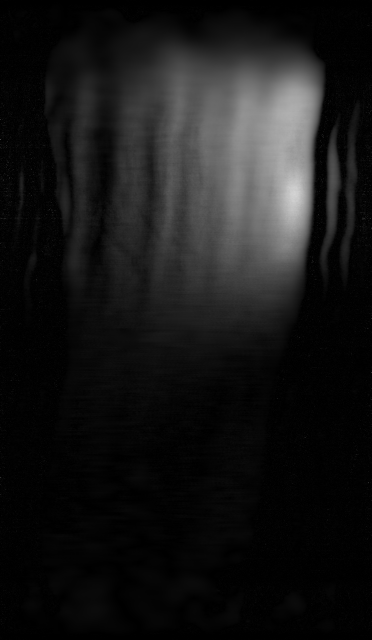
\includegraphics[width=.45\marginparwidth]{failure/coil_ims_01}
	\caption[Coil sensitivities in a failure case of the proposed algorithm]{%
		Under-smoothed coil sensitivities for the failure case of our algorithm in the third row and the second column of~\cref{fig:parallel imaging id}.%
	}%
	\label{fig:failure case coil sensitivities}
\end{sidefigure}
As a result, the reconstruction appears extremely smooth and anatomically implausible.
However, this can be corrected by appropriately choosing the respective regularization parameters, \( \mu \) and \( \lambda \) in~\cref{eq:joint inversion optimization problem}.\footnote{The details of our choice are in~\cref{ssec:details}.}
We never observed these types of failures when using our data-driven regularizer in the reconstruction algorithm and believe that they are extremely rare:
As indicated in~\cref{fig:mri sampling}, it prefers anatomically plausible structures over smooth images, facilitating the separation between the anatomy in the image and the coil sensitivities.

Finally, we analyze our proposed reconstruction algorithm with respect to the estimated coil sensitivities.
We consider the reconstruction problem shown in the first and third row of~\cref{fig:parallel imaging id}:
Cartesian frequency selection with acceleration \num{4}, and \qty{8}{\percent} and \qty{4}{\percent} autocalibration lines respectively.
As a reference offline estimation method, we chose the ESPIRiT algorithm~\cite{uecker_espirit_13}.
The estimated coil sensitivities for the \qty{8}{\percent} autocalibration lines reconstruction problem are shown in~\cref{fig:sensitivities}.
Due to the data fidelity term that we use in practice (see the discussion in~\cref{ssec:practical considerations}, in particular \cref{eq:data fidelity in practice}), the coil sensitivities from our estimation algorithm need not be pixel-wise normalized.
Hence, they look very physically plausible and match the reference well.
\begin{figure*}
	\begin{tikzpicture}
		\foreach [count=\isens] \senspath in {%
			ours,%
			espirit,%
			fully-sampled%
		}{%
			\node [inner sep=0, outer sep=0] (sens\isens) at (0, -\isens*2.2) {\foreach \idxx in {0,...,14}{%
				\includegraphics[rotate=180, width=\linewidth/15]{coil-estimates/\senspath/\idxx}%
			}};
		}
	\end{tikzpicture}
	\caption[Qualitative comparison of estimated coil sensitivities]{%
		Magnitude of the estimated sensitivities using our joint nonlinear inversion algorithm (top) versus the ESPIRiT~\cite{uecker_espirit_13} estimation (middle) for the reconstruction problem shown in the first row of~\cref{fig:parallel imaging id}.
		The bottom row shows the reference coil sensitivities computed with the fully-sampled data.
	}%
	\label{fig:sensitivities}
\end{figure*}

To better understand the quality of the estimation, we follow~\cite{uecker_espirit_13} and visualize the null-space residual in~\cref{fig:nullspace}.
As discussed in~\cref{ssec:methods pi}, any residual signal components indicate a suboptimal estimation of the coil sensitivities.
While the ESPIRiT estimation leads to slightly better results with \qty{8}{\percent} autocalibration lines, its performance deteriorates with only \qty{4}{\percent} autocalibration lines.
In contrast, our estimation remains stable, as the joint nonlinear inversion accounts for all available data, nut just autocalibration lines.
\begin{figure*}
	\centering
	\begin{tikzpicture}
		\def\cWidth{3.8cm}
		\def\chpad{2mm}
		\def\mhpad{5mm}
		\foreach [count=\i] \imname in {8percent/espi, 4percent/espi, 8percent/ours, 4percent/ours} {%
			\pgfmathsetlengthmacro{\xx}{\i * (\cWidth + \chpad) + (\i>2) * \mhpad}
			\node at (\xx, 0) {\includegraphics[rotate=180,width=\cWidth]{coil-estimates/null-space/\imname}};
			\pgfmathsetmacro{\annotation}{{"\qty{8}{\percent} ACLs","\qty{4}{\percent} ACLs"}[mod(\i+1,2)]}
			\node at (\xx, -3.55) {\small\annotation};
		}
		\foreach \anno/\xoff in {ESPIRiT/0cm, Ours/8.5cm}
		{
			\begin{scope}[xshift=\xoff]
				\draw [rounded corners, gray, thick] (1.9, -3.8) rectangle (10.1, 3.5);
				\node at (6, 3.7) {\small \anno};
				\pgfmathsetlengthmacro{\xx}{1 * (\cWidth + \chpad) - 0.3cm}
				\draw[-Stealth, ultra thick] (\xx, -1.5) -- ++(-.4, -.4);
				\pgfmathsetlengthmacro{\xxp}{2 * (\cWidth + \chpad) - 0.7cm}
				\draw[-Stealth, ultra thick] (\xxp, 1.0) -- ++(-.4, .3);
			\end{scope}
		}
	\end{tikzpicture}
	\caption[Null-space resudial of the estimated coil sensitivities]{%
		Qualitative comparison of the coil sensitivity estimation using the null-space residual:
		Any residual signal components point to a suboptimal estimation.
		We consider the Cartesian frequency selections with acceleration \num{4} in the first and third row of~\cref{fig:parallel imaging id}: \qty{8}{\percent} autocalibration lines and \qty{4}{\percent} autocalibration lines.%
		The proposed joint nonlinear inversion algorithm (right) provides superior estimates compared to offline estimation using ESPIRIT~\cite{uecker_espirit_13} (left) when little autocalibration data are available.
	}%
	\label{fig:nullspace}
\end{figure*}

\subsection{Generalization}%
\label{ssec:generalization}
A large part of this chapter was dedicated to designing a regularizer that can encode high-level features of the reference distribution.
We have demonstrated in~\cref{fig:mri sampling deep neural regularizers} that the regularizer (also due to the generative training) has indeed learned high-level features of the reference distribution.
In the previous sections we demonstrated thoroughly that utilizing the regularizer in a variational reconstruction framework leads to high-quality reconstructions for a variety problems where the underlying signal is a sample from the reference distribution.
In this section, we investigate how well our regularizer works for reconstruction problems where the underlying signal is \emph{not} a sample from the reference distribution.
Therefore, we consider three scenarios where the underlying signal is a
\begin{enumerate}
	\item \gls{corpdfs} \gls{mri} scan of a human knee, an
	\item \gls{mri} scan of a human brain, or an
	\item \gls{mri} examination of a prostate.
\end{enumerate}

In some sense, the items in the enumeration are increasingly out-of-distribution:
The fat-suppression---although it drastically changes the over-all appearance of the image---leaves edges at the same positions as the non-fat-suppressed scans and the image is still easily identified as a knee.
The brain scans are similar to the knee scans in the local structures appear similar and in that they have a region of almost all air around the region containing the signal, which is not the case for the prostate scans.
This is shown in~\cref{fig:ood spectrum}.
\begin{figure*}
	\begin{tikzpicture}
		\foreach [count=\ii] \impath/\annotation in {%
			{validation/cartesian/file1001057.h5/ground_truth}/{Knee (CORPD)},
			{validation-fs/cartesian/file1001916.h5/ground_truth}/{Knee (CORPDFS)},
			{scripts/ood/brain/reference-rss}/{Brain},
			{scripts/ood/prostate/reference-rss}/{Prostate}
		}
		{%
			\ifthenelse{\ii<3}{%
				\node at (\ii*4.2, 0) {\includegraphics[rotate=180,width=4cm]{\impath}};
			}{%
				\node at (\ii*4.2, 0) {\includegraphics[width=4cm]{\impath}};
			}
			\node at (\ii*4.2, 2.2) {\annotation};
		}
	\end{tikzpicture}
	\caption[Samples from the distributions considered in the out-of-distribution experiments]{%
		From left to right, the signals become increasingly different:
		The fat-suppressed knees retain the shape and edges.
		The brains local structures appear similar and it is surrounded by a region of almost zero-signal.
		The prostate scans appear completely different overall.
	}%
	\label{fig:ood spectrum}
\end{figure*}

First, we evaluate the data-driven regularizer on the fat-suppressed knee scans, following exactly the same setup as in the previous section.
In particular, we also evaluate the Charbonnier-smoothed isotropic \gls{tv} regularizer as well as the end-to-end \gls{vn} on this dataset.
We show qualitative qualitative results in~\cref{fig:parallel imaging ood}.
The corresponding quantitative results were already shown in~\cref{tab:parallel imaging}.
In summary, the quantitative results indicate our method generalizes slightly better to unseen data than the end-to-end \gls{vn} approach of~\cite{sriram_endtoend_2020}, although the performance degrades significantly in both cases.

In contrast to the end-to-end \gls{vn}, we can adapt the regularization strength to the new data.
To highlight the advantage of the tunable regularization parameters in our approach, we show results using the \( \lambda \)-fit (see~\cref{ssec:methods pi}) calculated on non-fat-suppressed data, as well as using parameters adapted to the task:
Obviously, the ability to tune the influence of the regularizer leads to improved performance when confronted with previously unseen data.
\begin{figure*}
	\centering
	\tikzexternaldisable
	\begin{tikzpicture}
		\def\cherries{{"file1001916.h5","file1000528.h5","file1000344.h5","file1001643.h5","file1000000.h5"}}
		\def\spyoff{{{0.05cm,0.0cm},{0.7cm,-0.4cm},{-0.7cm,0.1cm},{-0.4cm,.2cm},{-0.9cm,-0.4cm}}}
		\foreach [count=\isampling] \sampling/\sanno in {
			cartesian/Cartesian (\num{4}),
			{cartesian_rot90}/{Cartesian\textsuperscript{\qty{90}{\degree}} (\num{4})},
			{cartesian_4}/{Cartesian\textsuperscript{\qty{4}{\percent}} (\num{4})},
			gaussian2d/Gaussian (\num{8}),%
			radial/Radial (\num{11})%
		}{
			\pgfmathsetlengthmacro{\yy}{-\isampling * (\wwidth + \wwidth / 2 + \vpad)}
			\pgfmathsetmacro{\spyxoff}{\spyoff[\isampling-1][0]}
			\pgfmathsetmacro{\spyyoff}{\spyoff[\isampling-1][1]}
			\pgfmathsetmacro{\cherry}{\cherries[\isampling-1]}
			\foreach [count=\imethod] \method/\manno in {
				{zero_filled}/\glsxtrshort{zf},
				tv/\glsxtrshort{tv},
				vn/{\glsxtrshort{vn}},
				ours/{Ours \( \dagger \)},
				ours/{Ours \( * \)},
				ground_truth/Reference%
			}{
				\pgfmathsetlengthmacro{\xx}{\imethod * (\wwidth + \hpad)}
				\ifthenelse{\isampling=1}{\node at (\xx, -\wwidth / 2 - 1cm) {\manno};}{}
				\ifthenelse{\imethod=5}{
					\def\prefix{./figures/validation-fs-adapted}
				}{
					\def\prefix{./figures/validation-fs}
				}
				\pgfmathsetlengthmacro{\xxspy}{\xx + \spyxoff}
				\pgfmathsetlengthmacro{\yyspy}{\yy + \spyyoff}
				\coordinate (onn) at (\xxspy, \yyspy);
				\ifthenelse{\imethod=6}{}{
				\begin{scope}[mrispy]
					\node [inner sep=0, outer sep=0] at (\xx, \yy) {\includegraphics[angle=180,origin=c,width=\wwidth]{validation-fs/\sampling/\cherry/d_\method}};
					\spy on (onn) in node at (\xx + \wwidth / 2 / 2, \yy - 1.5 * \wwidth / 2);
				\end{scope}}
				\begin{scope}[mrispy]
					\node [inner sep=0, outer sep=0] at (\xx, \yy) {\includegraphics[angle=180,origin=c,width=\wwidth]{validation-fs/\sampling/\cherry/\method}};
					\spy on (onn) in node at (\xx - \wwidth / 2 / 2, \yy - 1.5 * \wwidth / 2);
				\end{scope}
			}
			\ifthenelse{\boolean{bPrintVersion}}{%
				\node [rotate=-90, overlay] at (19.0, \yy) {\sanno};
			}{%
				\node [rotate=90, overlay] at (1.2, \yy) {\sanno};
			}
		}
	\end{tikzpicture}
	\tikzexternalenable
	\caption[Qualitative results for parallel imaging on out-of-distribution data]{%
		Parallel imaging on out-of-distribution data.
		First row:
		Cartesian frequency selection with \qty{8}{\percent} autocalibration lines and acceleration \num{4}.
		Second row:
		As in the first row but with swapped phase encoding direction.
		Third row:
		As in the first row but with \qty{4}{\percent} autocalibration lines.
		Fourth row:
		2D Gaussian frequency selection with acceleration \num{8}.
		Fourth row:
		Radial frequency selection with acceleration \num{11}.
		The inlays show a detail zoom and the magnitude of the difference to the reference (\num{0}~\protect\drawcolorbar~\num{0.2}).
		The \( \dagger \) column shows the results using the regularization parameters from non-fat-suppressed data, the \( * \) column shows the results using adapted parameters.
	}%
	\label{fig:parallel imaging ood}
\end{figure*}

For the brain and prostate scan, we restrict ourselves to a setup as in~\cref{chap:regularizers};
the reference images and the data are shown in~\cref{fig:brain reference} and~\cref{fig:prostate reference} for the brain and the prostate scan respectively.
The scans are taken from the fastMRI brain dataset~\cite{9420272} and the fastMRI prostate dataset~\cite{tibrewala2024fastmri}.\footnote{%
	The images are the files \texttt{AXT1\_202\_2020190\_s8} (brain, eighth slice) and \texttt{AXT2\_013} (prostate).%
}
\begin{sidefigure}
	\centering
	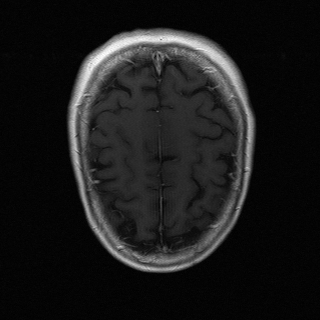
\includegraphics[width=\marginparwidth]{scripts/ood/brain/reference-rss}
	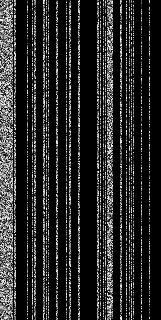
\includegraphics[width=.5\marginparwidth]{scripts/ood/brain/log-abs-data}
	\caption[Reference signal and zero-filled data for the brain scan]{The reference signal and the zero-filled data for the brain scan.}%
	\label{fig:brain reference}
\end{sidefigure}
\begin{sidefigure}
	\centering
	\includegraphics[width=\marginparwidth]{scripts/ood/prostate/reference-rss}
	\includegraphics[width=.5\marginparwidth]{scripts/ood/prostate/log-abs-data}
	\caption[Reference signal the zero-filled data for the prostate scan]{The reference signal and the zero-filled data for the prostate scan.}%
	\label{fig:prostate reference}
\end{sidefigure}

We show the reconstructions depending on the regularization parameter in~\cref{fig:brain prostate recos}.
\begin{figure*}
	\centering
	\begin{tikzpicture}
		\foreach [count=\ia] \anatomy in {brain, prostate}{%
			\pgfmathsetlengthmacro{\yy}{-\ia * (\wwidth + 2mm)}
			\foreach [count=\ir] \regweight/\llabel in {0.00/ZF, 0.10/\( \lambda = \num{0.1}\), 1.00/\num{1}, 10.00/\num{10}, 100.00/\num{100}, 1000.00/\num{1000}}{%
				\pgfmathsetlengthmacro{\xx}{\ir * (\wwidth + \hpad)}
				\node at (\xx, \yy) {\includegraphics[width=\wwidth]{scripts/ood/\anatomy/rec_\regweight.png}};
				\ifthenelse{\ia=1}{
				\node at (\xx, \yy + 1.5cm) {\llabel};}{}
			}
		}
	\end{tikzpicture}
	\caption[Simulation study on out-of-distribution signals]{%
		Simulation study on out-of-distribution signals:
		When the underlying signal is an \gls{mri} scan of the brain, the regularizer yields reasonable solutions.
		When the underlying signal is an \gls{mri} scan of the prostate, it tries to impart knee-like structure, especially at the boundaries.
	}%
	\label{fig:brain prostate recos}
\end{figure*}
The reconstructions of the brain appear reasonable, with the reconstruction becoming smoother as the regularization becomes stronger.
The reconstructions of the prostate have knee-like structures, especially at the boundary.
These boundary effects deserve more investigation and highlight that the regularizer is only expected to work well when the underlying signal is from the distribution it models.
\section{Discussion}%
\label{sec:discussion}
This chapter's first part focused on designing an architecture suitable for modeling the negative log-prior.
Unlike classical regularizers used in imaging applications, the regularizer is \emph{not} translation invariant and can model non-local dependencies.
Coupled with a generative learning approach, the data-driven regularizer encodes high-level domain statistics as demonstrated by synthesizing realistic knee \glspl{mri} without any data (see \cref{fig:mri sampling}).
Consequently, reconstructions from severely ill-posed problems, such as \gls{mri} with a random frequency selection and acceleration \num{3}, appear natural.

Using a joint nonlinear inversion algorithm, we achieved state-of-the-art reconstructions in clinically relevant parallel \gls{mri} settings.
The strict separation of likelihood and prior, combined with our generative learning approach, ensures stable reconstruction quality across various frequency selection, as shown in~\cref{fig:parallel imaging id}.
This is a significant advantage over traditional methods, where reconstruction quality often depends on specific frequency selections, such as phase encoding direction, which may need to be adjusted when encountering problematic blood vessel positions.
Our regularizer does not require retraining for new advantageous frequency selections.

Our regularizer also performs well in out-of-distribution experiments, underscoring the importance of controlling its influence.
\cref{tab:parallel imaging} shows that adjusting regularization strength to the underlying data strongly improves performance.
Regularization strength was tuned for Cartesian frequency selection with \qty{8}{\percent} autocalibration lines (see~\cref{ssec:methods pi}) and acceleration \num{4}.
Results for the radial frequency selection indicate a sub-optimal fit for the out-of-distribution data.
The fit on the \gls{corpd} data (\( \dagger \) column) performs better than the fit calculated on \gls{corpdfs} data.
\cref{fig:parallel imaging ood} suggests that the adapted parameters lead to an over-smoothed reconstruction, which could be improved by adapting the regularization strength to the \gls{corpdfs} data \emph{and} the radial frequency selection.
Generally, adapting the regularization strength to the frequency selection and the data is beneficial, but typically not possible with other data-driven approaches.

The probabilistic interpretation of our approach is significant in two ways:
First, the regularizer can be inspected through data-independent analysis (see \cref{fig:mri sampling}) allowing experts to visualize preferred structures and improving clinician confidence in reconstructions.
Second, since any datum provides a posterior distribution of reconstructions, we can compute compute pixel-wise marginal variances, offering clinicians additional information.
For example, \cref{fig:simulation study posterior sampling} shows high variance around small anatomic structures, suggesting clinicians might need more information if decisions are based on these areas.
Most other data-driven approaches only provide a point estimate.

Experiments on synthetic single-coil data show the \gls{mmse}'s quantitative and qualitative superiority of over the \gls{map} estimate.
In light of the introductory chapter this is not surprising, but in addition to the rational outlined there we believe that this is related to the training procedure:
During training, the regularizer encounters slightly noisy images in the Langevin process (see~\cref{ssec:methods ml}), and injecting the same noise in the reconstruction algorithm improves performance.
However, this performance improvement does not translate to parallel imaging experiments, possibly because our joint nonlinear inversion biases the reconstruction such that this effect is no longer observable.

Our parallel \gls{mri} reconstruction algorithm is fast:
\cref{alg:ipalm} converges in around \num{100} iterations, taking around \qty{5}{\second} on an NVIDIA Titan RTX using approximately \qty{2}{\giga\byte} of memory.
This contrasts with diffusion models where reconstruction times of up to \qty{10}{\minute} are reported~\cite{chung_scoremri_2022}.
Speed is advantageous in practice, allowing images to be viewed while the patient is still in the scanner and enabling immediate adjustments to the frequency selection if needed.

\section{Conclusion}%
\label{sec:conclusion deep neural regularizer}
We leverage modern generative learning techniques to train a regularizer that faithfully encodes the underlying distribution of the training data.
Embedding this regularizer in a variational reconstruction framework enables satisfactory reconstruction of both single-coil and parallel \gls{mri} by adapting the data fidelity term.
Quantitative and qualitative analyses show that our approach achieves competitive reconstruction performance, matching or surpassing discriminative approaches.
Furthermore, our approach is robust to changes in the frequency selection, while the discriminative reference methods introduce severe hallucinations when confronted with previously unseen data.
The anatomical knowledge encoded in our regularizer allows us to reconstruct high quality images even from random sampling masks.
On out-of-distribution data, our method performs as well as or better than hand-crafted regularizers such as \gls{tv} or other discriminative methods, demonstrating superior generalization to distribution shifts.

Our method also provides a natural accompanying probabilistic interpretation through statistical modeling and Bayesian inference.
This allows experts to explore a distribution of reconstructions, whereas other data-driven approaches typically provide only point estimates.
Experiments suggest that this distribution encodes important diagnostic information, such as high uncertainty around small anatomical structures, potentially aiding clinical decision making.
Additionally, we can perform a data-independent analysis of the model by visualizing the Gibbs distribution, providing insight into the information encoded in the regularizer unlike the black-box nature of other data-driven methods.

For parallel \gls{mri} reconstruction, we propose a fast algorithm that jointly estimate the image and the coil sensitivities.
Unlike offline sensitivity estimation, our approach does not require autocalibration lines, can be applied to non-Cartesian sampling trajectories and nonuniform sampling, and utilizes all available data.
The resulting optimization problem can be solved efficiently using non-convex optimization algorithms, delivering high quality reconstructions in approximately \qty{5}{\second} on consumer hardware.

We believe that reconstruction approaches based on generative priors hold significant potential.
A natural extension of our work would be to combine the image-prior with a learned sensitivity-prior.
Future research could also explore enhancing the simple architecture used in this paper with more modern building blocks, such as attention layers.
Additionally, investigating whether local convolutional models can replicate the performance of our generative prior is a promising direction for further study.
